% This must be in the first 5 lines to tell arXiv to use pdfLaTeX, which is strongly recommended.
\pdfoutput=1
% In particular, the hyperref package requires pdfLaTeX in order to break URLs across lines.

\documentclass[11pt]{article}

% Change "review" to "final" to generate the final (sometimes called camera-ready) version.
% Change to "preprint" to generate a non-anonymous version with page numbers.
\usepackage[preprint]{acl}

% Standard package includes
\usepackage{times}
\usepackage{latexsym}

% For proper rendering and hyphenation of words containing Latin characters (including in bib files)
\usepackage[T1]{fontenc}
% For Vietnamese characters
% \usepackage[T5]{fontenc}
% See https://www.latex-project.org/help/documentation/encguide.pdf for other character sets

% This assumes your files are encoded as UTF8
\usepackage[utf8]{inputenc}

% This is not strictly necessary, and may be commented out,
% but it will improve the layout of the manuscript,
% and will typically save some space.
\usepackage{microtype}

% This is also not strictly necessary, and may be commented out.
% However, it will improve the aesthetics of text in
% the typewriter font.
\usepackage{inconsolata}

%Including images in your LaTeX document requires adding
%additional package(s)
\usepackage{graphicx}
\usepackage{subcaption}
\usepackage{booktabs}

% If the title and author information does not fit in the area allocated, uncomment the following
%
%\setlength\titlebox{<dim>}
%
% and set <dim> to something 5cm or larger.

\title{QUACLRS: QUasi-supervised Audio Classification by Learning Representations from Spectrograms}

% Author information can be set in various styles:
% For several authors from the same institution:
\author{Arya Shah, Aman Oberoi \\
         Department of Computer Science and Information Management\\ Asian Institute of Technology \\ Pathumthani, Thailand \\ \texttt{{{st125462, st125490}@ait.ac.th}}}
% if the names do not fit well on one line use
%         Author 1 \\ {\bf Author 2} \\ ... \\ {\bf Author n} \\
% For authors from different institutions:
% \author{Author 1 \\ Address line \\  ... \\ Address line
%         \And  ... \And
%         Author n \\ Address line \\ ... \\ Address line}
% To start a separate ``row'' of authors use \AND, as in
% \author{Author 1 \\ Address line \\  ... \\ Address line
%         \AND
%         Author 2 \\ Address line \\ ... \\ Address line \And
%         Author 3 \\ Address line \\ ... \\ Address line}

%\author{Arya Shah \\
  %Department of Computer Science and Information Management \\
  %Asian Institute of Technology\\
  %Pathumthani, Thailand \\
  %\texttt{st125462@ait.ac.th} \\\And
  %Second Author \\
  %Affiliation / Address line 1 \\
  %Affiliation / Address line 2 \\
  %Affiliation / Address line 3 \\
  %\texttt{email@domain} \\}

%\author{
%  \textbf{First Author\textsuperscript{1}},
%  \textbf{Second Author\textsuperscript{1,2}},
%  \textbf{Third T. Author\textsuperscript{1}},
%  \textbf{Fourth Author\textsuperscript{1}},
%\\
%  \textbf{Fifth Author\textsuperscript{1,2}},
%  \textbf{Sixth Author\textsuperscript{1}},
%  \textbf{Seventh Author\textsuperscript{1}},
%  \textbf{Eighth Author \textsuperscript{1,2,3,4}},
%\\
%  \textbf{Ninth Author\textsuperscript{1}},
%  \textbf{Tenth Author\textsuperscript{1}},
%  \textbf{Eleventh E. Author\textsuperscript{1,2,3,4,5}},
%  \textbf{Twelfth Author\textsuperscript{1}},
%\\
%  \textbf{Thirteenth Author\textsuperscript{3}},
%  \textbf{Fourteenth F. Author\textsuperscript{2,4}},
%  \textbf{Fifteenth Author\textsuperscript{1}},
%  \textbf{Sixteenth Author\textsuperscript{1}},
%\\
%  \textbf{Seventeenth S. Author\textsuperscript{4,5}},
%  \textbf{Eighteenth Author\textsuperscript{3,4}},
%  \textbf{Nineteenth N. Author\textsuperscript{2,5}},
%  \textbf{Twentieth Author\textsuperscript{1}}
%\\
%\\
%  \textsuperscript{1}Affiliation 1,
%  \textsuperscript{2}Affiliation 2,
%  \textsuperscript{3}Affiliation 3,
%  \textsuperscript{4}Affiliation 4,
%  \textsuperscript{5}Affiliation 5
%\\
%  \small{
%    \textbf{Correspondence:} \href{mailto:email@domain}{email@domain}
%  }
%}

\begin{document}
\maketitle
\begin{abstract}
Environmental sound classification faces significant challenges including limited labeled data, restricted class diversity, and inconsistent performance in noisy environments. This research introduces QUACLRS, a quasi-supervised framework that enhances audio classification through representation learning from spectrograms. We extend the UrbanSound8K dataset with four additional urban sound classes (ambulance, firetruck, police, traffic) and implement specialized audio augmentation techniques including time stretch, pitch shift, SpecAugment, and PatchAugment. Our methodology systematically evaluates various CNN architectures (ResNet, MobileNet, EfficientNet, ConvNext, VGG16, InceptionNet) and self-supervised learning approaches (SimCLR, MoCo, BYOL, BarlowTwins, DINO, SwAV) using k-fold cross-validation. Experimental results demonstrate that EfficientNet achieves the highest classification accuracy (82.09\%) among pretrained models, while models trained from scratch consistently outperform their pretrained counterparts by an average of 3.12 percentage points. Among self-supervised learning techniques, SimCLR demonstrates superior performance (65\% accuracy) followed by MoCoV2 (62\%) and MoCo (60\%). Our findings reveal that audio-specific augmentations significantly enhance model robustness, with PatchAugment showing the most consistent improvements. This research advances environmental sound classification by developing techniques that maximize performance with limited labeled data while providing valuable insights into effective representation learning for audio data.
\end{abstract}

\section{Introduction}

Environmental sound classification faces critical challenges including limited labeled data, restricted class diversity, and inconsistent performance in noisy environments. Current audio classification systems often struggle with generalizability across diverse acoustic environments and require significant amounts of labeled data to achieve acceptable performance. In particular, common benchmark datasets such as UrbanSound8K contain limited class diversity, constraining the development of robust audio classification models.

The ability to accurately classify environmental sounds has significant applications across numerous domains including urban monitoring, security surveillance, assistive technologies, and multimedia content analysis. With the proliferation of audio-enabled IoT devices and smart city initiatives, robust audio classification systems that can operate effectively with limited labeled data and in diverse acoustic environments are increasingly important. Recent advances in self-supervised learning techniques have shown promise in vision domains but remain underexplored for audio classification tasks.

This research introduces a comprehensive framework that combines:

\begin{enumerate}
    \item An extended version of the UrbanSound8K dataset with additional urban sound classes (ambulance, firetruck, police, traffic) and specialized audio augmentation techniques (time stretch, pitch shift, SpecAugment, PatchAugment)
    \item A modular CNN architecture for spectral feature extraction, exploring various backbones (ResNet, MobileNet, EfficientNet, ConvNext, VGG16, InceptionNet)
    \item Self-supervised learning techniques adapted for spectrograms, including contrastive methods (SimCLR, MoCo, BYOL) and non-contrastive approaches (DINO, BarlowTwins)
    \item A systematic evaluation methodology using k-fold cross-validation to assess model robustness and generalizability
\end{enumerate}
We observe that our extended dataset combined with audio-specific data augmentation techniques will demonstrate significant improvements in classification performance, particularly when paired with self-supervised learning approaches. We expect to observe: (1) improved model robustness to noise and domain shifts, (2) enhanced generalizability across diverse environmental sound classes, (3) reduced dependency on large volumes of labeled data, and (4) identification of optimal combinations of CNN architectures and self-supervised learning techniques for audio event classification.

This research advances the field of environmental sound classification by developing techniques that maximize performance with limited labeled data. By extending dataset diversity and implementing specialized augmentation techniques, we address fundamental challenges in audio classification. Our integration of state-of-the-art self-supervised learning approaches provides valuable insights into effective representation learning for audio data. The proposed framework demonstrates a practical path toward more robust and generalizable audio classification systems, with potential applications across diverse domains requiring acoustic scene understanding.
\begin{figure}
    \centering
    \includegraphics[width=1\linewidth]{latex/assets/dataset_extension_process.PNG}
    \caption{Placehoder for first figure illutstration 1}
    
\end{figure}
Throughout our research, our aim has been to answer the following formulated research questions, to answer, which we believe are crucial for the outcome of our study:

\textbf{RQ 1}: How can self-supervised learning techniques improve audio event classification performance with limited labeled data? 

\textbf{RQ 2}: To what extent can specialized data augmentation techniques enhance the robustness of audio classification models in noisy environments? 

\textbf{RQ 3}: How does expanding existing audio datasets with additional diverse classes affect the generalizability and robustness of sound event classification models?

\textbf{RQ 4: }What combination of semi-supervised learning techniques and data augmentation strategies yields the most effective performance improvements for environmental sound classification tasks?

\section{Related Work}

In the domain of audio processing and classification, traditional supervised learning approaches have demonstrated remarkable success. However, these methods typically require large amounts of labeled data, which can be time-consuming, expensive, and sometimes infeasible to obtain in specialized domains like bioacoustics, medical audio analysis, and environmental sound monitoring. With the growing need to address challenges related to data scarcity in audio domains, self-supervised learning (SSL) has emerged as a promising paradigm that enables models to learn meaningful representations from unlabeled data, which can then be fine-tuned for downstream tasks with limited labeled examples.

\subsection{Self-Supervised Learning for Audio Classification}

\subsubsection{Contrastive Learning Approaches}

Contrastive learning has emerged as a powerful approach for self-supervised representation learning in audio domains \citep{moummad2024selfsupervisedlearningfewshotbird} evaluated three main self-supervised learning approaches for bird sound classification: SimCLR (sample contrastive learning), Barlow Twins (dimension contrastive learning), and FroSSL (combining both sample and dimension contrastive learning). Their research revealed that Barlow Twins achieved superior performance with 48.90\% accuracy on 5-way 1-shot tasks, outperforming the CNN14 inference baseline's 43.69\%. A key innovation in their work was the use of window selections optimized for bird activations using a pretrained audio neural network (PANN), which significantly boosted performance across all methods. When PANN selection was applied to both training and testing phases for SimCLR, accuracy increased dramatically from 43.28\% to 64.19\%. However, the authors noted that supervised contrastive learning still outperformed SSL approaches with 73.07\% accuracy, indicating room for improvement in purely self-supervised techniques.
Building on contrastive learning principles, \citep{guzhov2021audioclipextendingclipimage} introduced AudioCLIP, which extends the Contrastive Language-Image Pre-training (CLIP) framework to incorporate audio as a third modality alongside text and images. By combining an ESResNeXt audio encoder with text and image encoders from CLIP, AudioCLIP established new benchmarks for environmental sound classification, achieving 90.07\% accuracy on UrbanSound8K and 97.15\% on ESC-50. Notably, AudioCLIP also demonstrated impressive zero-shot classification capabilities with 68.78\% and 69.40\% accuracy on these datasets respectively, significantly outperforming previous approaches like VGGish+Word2Vec+GloVe which achieved only 33.00\% on ESC-50. This work highlighted the potential of multimodal learning and cross-modal querying for audio tasks, although some performance degradation was observed on ImageNet tasks after AudioSet training, suggesting challenges in balancing multi-domain learning.
Contrastive learning has also been adapted for specialized audio domains. [Patch-Mix Contrastive Learning with Audio Spectrogram Transformer on Respiratory Sound Classification, 2023] proposed a patch-level mixing technique combined with contrastive learning for respiratory sound classification using an Audio Spectrogram Transformer (AST). Their method randomly replaces patches in spectrograms with those from other samples and employs a contrastive learning framework to distinguish mixed representations in the latent space. When applied to the ICBHI 2017 Respiratory Sound Database, this approach achieved a state-of-the-art score of 62.37\%, outperforming previous methods by 4.8\%. The authors demonstrated that pre-training on both visual (ImageNet) and audio (AudioSet) domains enhanced generalization for respiratory sounds, although they acknowledged limitations in model interpretability and computational requirements analysis.
In the context of noisy environments, \citep{app14219711} introduced a Contrastive Learning-based Audio Spectrogram Transformer (CL-Transformer) framework that combines feature fusion of original and noisy signal information with optimized contrastive learning. This approach maintained high accuracy rates of 88.65\% and 91.28\% on UrbanSound8K with white Gaussian noise at 0dB and 10dB SNR, demonstrating exceptional resistance to noise interference. Overall, their framework achieved 97.75\% accuracy on ESC-50 and 92.95\% on UrbanSound8K, outperforming numerous existing methods. However, the authors noted that the method's effectiveness in real urban environments might be limited due to the complexity of actual audio conditions beyond simple white noise.

\subsubsection{Alternative Self-Supervised Learning Approaches}

Beyond contrastive learning, researchers have explored various alternative self-supervised learning strategies. \citep{TRIPATHI2021108183} proposed an innovative approach using data augmentation recognition as a pretext task for environmental sound classification. Their SpectroLab Outfits framework trained a ResNet-18 model to distinguish between three types of data augmentations (Time Shifting, Change in Speed, SpecAugment) applied to audio signals. This approach achieved 91.67\% accuracy on ESC-10 and 75.09\% accuracy on DCASE 2019 Task-1(A), outperforming the PiczakCNN baseline with 19.84 million fewer parameters. The authors provided extensive empirical data inspections through visualization tools like t-SNE plots and GRAD-CAM, demonstrating the effectiveness of their augmentation-based pretext task. However, they acknowledged limitations in the variety of augmentation methods explored and noted persistent confusion between acoustically similar classes.
For anomalous sound detection (ASD) in machine condition monitoring, \citep{wilkinghoff2023selfsupervisedlearninganomaloussound} introduced FeatEx, a self-supervised method that implements an embedding exchange mechanism within a two-branch framework. FeatEx selects two training samples and creates a new embedding by combining the first sub-network embedding from one sample with the second sub-network embedding from another, forcing the model to determine when different sub-network embeddings should pair up. Evaluated on DCASE2022 and DCASE2023 ASD datasets, FeatEx surpassed baseline approaches and other SSL methods, particularly when supervised training loss was integrated with SSL losses. The approach established new state-of-the-art performance on DCASE2023 ASD, although the authors noted that the implementation requires a specific two-branch architecture, potentially limiting its applicability with other network designs.
In contrast to representation learning approaches, \citep{CHEN2025110593} explored metric learning for environmental sound classification through their SoundMLR framework. By combining an Adaptive Sparse Pairwise (AdaSP) metric loss with cross-entropy loss and introducing Spectral Pooling Attention and Feature Pooling modules to optimize a MobileNetV2 backbone, SoundMLR achieved accuracies of 91.91\%, 90.75\%, and 85.22\% on ESC-51, ESC-50, and UrbanSound8k respectively. A key advantage of this approach was its computational efficiency, with an inference latency of just 4.46ms, making it suitable for near real-time applications. The Feature Pooling Layer Module reduced computational complexity by 24.5\% while improving accuracy to 92.16\% on ESC-51. However, the authors observed inconsistent performance across datasets, with SoundMLR showing greater improvements on ESC-50/51 than on UrbanSound8k, suggesting potential generalization challenges.

\subsection{End-to-End Approaches and Architectural Innovations}

\subsubsection{Raw Waveform Processing}
While many audio classification approaches utilize spectrograms or pre-extracted features, \citep{abdoli2019endtoendenvironmentalsoundclassification} proposed an end-to-end solution using 1D Convolutional Neural Networks (CNNs) that operate directly on raw audio waveforms. Their compact design, containing only 3-5 convolutional layers with large receptive fields in the initial layers, achieved an impressive 89\% mean accuracy on the UrbanSound8k dataset, surpassing other methods by 11-27\%. With only 550,000 parameters, compared to 101 million in models like EnvNet-v2, their approach required less training data while eliminating the need for feature extraction or data augmentation. The first convolutional layer, optionally initialized with a Gammatone filterbank to simulate human auditory functions, learned filters that mirrored human auditory perception in a logarithmic manner. Using a sliding window method, the model could process audio signals of arbitrary length, although some performance limitations were observed between specific sound classes like "Street music" and "Children playing."

\subsubsection{Novel Detection Frameworks}
Extending beyond classification to detection tasks, \citep{Venkatesh_2022} introduced "You Only Hear Once" (YOHO), a YOLO-like algorithm for audio segmentation and sound event detection. YOHO utilizes regression to predict the boundaries of acoustic events, treating them as temporal "bounding boxes" analogous to the spatial bounding boxes in computer vision. Implemented with a MobileNet architecture using depthwise followed by pointwise convolution, YOHO demonstrated superior performance compared to CRNN models on most datasets, including DCASE 2017 and URBAN-SED. The approach's computational efficiency and scalability, coupled with the paradigm shift from temporal classification to boundary regression, provided greater flexibility for working with various audio tasks. However, the authors acknowledged limitations in handling overlapping sounds within a detected time range and potential misalignments due to regression-based boundary prediction.
Taking a different approach to detection tasks, \citep{8995448} leveraged the Mask-RCNN framework for robust sound event detection, particularly for rare events like glass breaks or baby cries. Their unified network combined temporal and spatial aspects to localize events by placing window bounding boxes around spectrogram regions. Using a ResNet-101 backbone and ROI-Align for pixel-to-pixel level alignment, the model integrated frame-level classification through 1D CNN blocks with batch normalization, ReLU activation, and max pooling. While effective for event occurrence detection, the authors noted that the fixed height of generated bounding boxes limited the model's ability to separate sounds from multi-source events.

\subsubsection{Multimodal and Source Separation Approaches}
For tasks requiring source separation, \citep{kadandale2020multichannelunetmusicsource} proposed a multi-channel U-Net for music source separation as an alternative to conventional U-Net architectures. Unlike Conditional U-Net (C-UNET) which uses conditioning in the control flow, their Multi-channel U-Net (M-U-Net) employed a multi-task loss with Dynamic Weight Averaging and Energy-based Weighting methods to balance focus between higher and lower energy instruments. With fewer parameters and training epochs required, M-U-Net demonstrated efficient performance on the MUSDB18 dataset, though questions remained about its generalization capabilities in varying environments with difficult-to-distinguish overlapping sources.

Expanding the boundaries of universal sound separation, \citep{zhao2024universalsoundseparationselfsupervised} developed a system incorporating Sound Event Detection (SED), query-based source separation, and latent source embedding processes. Leveraging self-supervised learning through a Masked Audio Encoder (MAE) that replaced the typical U-Net for mixture prediction, their approach utilized pretrained models like VGG for clean sound source detection from weakly labeled data. A key innovation was their energy-based augmentation technique that preserved distribution while applying modifications. Building on anchor segment mining and hierarchical token-semantic auto-transformer concepts (swim-transformers), the system demonstrated potential for handling a wide range of sounds across speech, music, and environmental monitoring domains, though the authors acknowledged that more ablation studies were needed to prove the robustness of learned representations.

For audio representation at the signal level, \citep{vu2024endtoendinterpretableconvolutionalneural} investigated interpretable convolutional neural networks for waveform signals by incorporating varying learnable window size filters, including SincNet and Gaussian filters. By parameterizing window functions based on filter shape and frequency gain, their approach captured end-to-end solutions from raw sound signals with minimal feature engineering. The model, initialized using Mel frequency at lower frequency bands to capture speech signals, consisted of two layers with 512 nodes and layer normalization. This approach provided better interpretability and transparency while directly working with waveforms, potentially preventing signal shifts. Tested on emotional speech datasets CREMA-D and IEMOCAP, the method demonstrated the value of incorporating domain knowledge while maintaining controllability through learning crucial parameters and time domain dynamics.

\subsection{Specialized Domain Applications}

\subsubsection{Bioacoustics}
In the field of bioacoustics, \citep{https://doi.org/10.1049/cit2.12007} addressed the challenge of detecting unknown bird species and individuals using a generative autoencoder architecture. Their approach combined discriminative (identifying temporal boundaries) and non-discriminative (characterizing each class independently) elements, utilizing latent representations of log mel frequency spectrograms for comparison in the frequency domain rather than the time domain. Applied to North American Bird species data comprising 2,762 known and 339 anonymous bird sound samples, their simple architecture demonstrated potential for characterizing voice features from unlabeled data, although questions remained about the impact of normal distribution assumptions in the VAE latent space on the fat-tailed distributions typical of low mel frequencies. 

\subsubsection{Medical Acoustics}
\citep{Bae_2023} applied self-supervised learning to respiratory sound classification for diagnosing lung diseases, addressing both the scarcity of medical data and the limitations of conventional augmentation techniques for datasets with hierarchical class structures. Using an Audio Spectrogram Transformer (AST) pretrained on both ImageNet and AudioSet in a transfer learning setting, combined with their novel patch-level mixing technique and contrastive learning framework, they achieved a state-of-the-art score of 62.37\% on the ICBHI dataset, improving upon previous methods by 4.8\%. While demonstrating that pre-training on both visual and audio domains enhanced generalization, the authors noted limitations in model interpretability and computational requirement analysis, which are particularly important for medical applications where understanding model decisions is crucial for clinical acceptance.

\subsubsection{Environmental Sound Classification}
Environmental sound classification has been approached from multiple angles, with several papers demonstrating innovations in this space. \citep{TRIPATHI2021108183} addressed the challenge using their data augmentation recognition pretext task, achieving 91.67\% accuracy on ESC-10 and 75.09\% on DCASE 2019 Task-1(A) with fewer parameters than baseline models. \citep{abdoli2019endtoendenvironmentalsoundclassification} took an end-to-end approach using 1D CNNs directly on audio waveforms, reaching 89\% accuracy on UrbanSound8k while eliminating the need for feature extraction.\citep{guzhov2021audioclipextendingclipimage} extended the multimodal capabilities through AudioCLIP, achieving 90.07\% on UrbanSound8K and 97.15\% on ESC-50, with impressive zero-shot classification performance. \citep{app14219711} focused on robustness in noisy environments, maintaining high accuracy even with significant noise interference. Most recently, \citep{CHEN2025110593} demonstrated the potential of metric learning with their SoundMLR framework, balancing accuracy with computational efficiency for near real-time applications.

\subsubsection{Anomalous Sound Detection}
For machine condition monitoring, \citep{wilkinghoff2023selfsupervisedlearninganomaloussound} introduced FeatEx as a self-supervised approach to anomalous sound detection. Evaluated on DCASE2022 and DCASE2023 ASD datasets derived from ToyAdmos2 and MIMII-DG, FeatEx outperformed baseline approaches and other SSL methods, particularly on the DCASE2023 dataset where simpler classification tasks maximized SSL benefits. The authors established new state-of-the-art performance on DCASE2023 ASD through extensive ablation tests demonstrating the validity of their design decisions regarding SSL losses applied with class labels and trainable center classes alongside temporal mean normalization. However, they acknowledged limitations in computational efficiency and the method's dependence on a specific two-branch architecture.

\subsection{Gaps and Future Directions}
\citep{moummad2024selfsupervisedlearningfewshotbird} highlighted that bird-specific invariances remain understudied, with most approaches employing domain-agnostic data augmentation rather than exploring phenomena specific to bird vocalizations. They suggested future work should focus on bird-specific acoustic properties and methods for tracking temporal patterns in vocalizations, along with developing automatic window selection capabilities that operate without pre-trained supervised models. \citep{TRIPATHI2021108183} identified opportunities to explore a wider range of augmentation methods beyond the three techniques (Time Shifting, Change in Speed, SpecAugment) used in their study, as well as investigating different pretext tasks such as spectrogram segment order prediction and partial reconstruction. They also noted potential benefits from integrating various SSL approaches, such as combining their augmentation recognition method with contrastive learning techniques.\citep{wilkinghoff2023selfsupervisedlearninganomaloussound} emphasized the need for more efficient computational methods in combined SSL systems and suggested evaluating SSL techniques from speech and audio fields, including BYOL for audio applications with contrastive learning. They also recommended assessing how embeddings produced through SSL techniques might transfer across different downstream processing operations. \citep{Bae_2023} pointed to the importance of incorporating attention visualization and other interpretability techniques for medical applications, allowing clinicians to better understand model decision processes. They also suggested investigating self-supervised pre-training on respiratory sounds as an additional approach to enhance performance given limited labeled data. \citep{app14219711} highlighted the need to study more complex noise types beyond white Gaussian noise and develop methods to mitigate destructive elements from flexible audio components like thunder and winds. They also suggested exploring multi-modal approaches combining visual, contextual, and audio elements for improved classification outcomes. \citep{CHEN2025110593} identified opportunities to extend their approach to handle longer audio recordings and investigate how well learned representations transfer across different audio domains. They also suggested developing specialized techniques to address class imbalance in datasets like UrbanSound8k.\citep{abdoli2019endtoendenvironmentalsoundclassification} proposed investigating the combination of 1D and 2D representation methods to leverage complementary effects, enhancing performance for difficult sound classes, and exploring attention-based components or transformers for improved temporal dependency detection. \citep{guzhov2021audioclipextendingclipimage} recommended replacing image and audio encoders with updated, more powerful networks and developing methods to reduce performance degradation on ImageNet after AudioSet training. They also suggested investigating few-shot learning capabilities and improved methods for understanding temporal patterns in audio for event identification. \citep{8995448} pointed to the limitations of fixed bounding box heights in their Mask-RCNN approach, suggesting future work could enhance the model's ability to separate sounds from multi-source events. \citep{Venkatesh_2022} noted that YOHO's performance on the TUT Sound Event Detection dataset lagged behind other datasets, suggesting potential for improvement through boundary-level augmentation techniques and architectural modifications like adding more layers or incorporating ResNet skip connections.
\section{Dataset}
\begin{figure*}
  \centering
  \includegraphics[width=\textwidth]{latex//assets/dataset_extension_process.PNG}
  \caption{The Dataset Extension Process Pipeline}
  
\end{figure*}

For our research, we will be focusing on our extension of the UrbanSound8K dataset. Our extended dataset enhances the original collection with additional urban sound classes and implements specialized audio augmentation techniques to improve model robustness and generalizability. The original UrbanSound8K dataset is a widely used benchmark in environmental sound classification research. It contains 8,732 labeled sound excerpts (less than or equal to 4 seconds) totaling approximately 7.3 hours of audio and comprises 10 classes: air conditioner, car horn, children playing, dog bark, drilling, engine idling, gunshot, jackhammer, siren, and street music which is organized into 10 pre-defined folds for cross-validation. Most classes have approximately 1,000 samples (air conditioner, children playing, dog bark, drilling, engine idling, jackhammer, street music). Some classes have fewer samples: car horn (429), gun shot (374), and siren (929).
The dataset extension process involved a comprehensive approach to incorporate new audio classes while ensuring data quality and consistency. We expanded the dataset by adding four new urban sound categories from the sireNNet directory: ambulance (400 samples), firetruck (400 samples), police (454 samples), and traffic (421 samples). These additions significantly enriched the dataset's representation of emergency and urban environmental sounds. Audio preprocessing was a critical step to standardize the dataset. All recordings were normalized to a uniform duration of 4 seconds, which established consistency across samples. We implemented a 48kHz sample rate resampling to ensure high-quality audio representation. For recordings shorter than the standard duration, silence padding was applied to reach the 4-second mark, while longer recordings were trimmed from the center to maintain the most relevant acoustic information. To prepare the audio data for machine learning applications, we converted all audio files into mel spectrograms using the librosa library. Mel spectrograms are visual representations of sound that emphasize frequencies according to human auditory perception, making them particularly suitable for audio classification tasks. The transformation utilized specific parameters: a Fast Fourier Transform (n\_fft) size of 2048, a hop length of 512, and 128 mel bands. The frequency range was constrained between 20Hz and 8000Hz to capture the most relevant acoustic information while reducing computational requirements.
To enhance dataset robustness and prevent overfitting, we implemented multiple augmentation techniques:
\begin{enumerate}
    \item \textbf{Time Stretch}: This technique modified the playback speed of audio samples (at 0.8x and 1.2x rates) without affecting pitch characteristics, simulating variations in sound source speeds.
    \item \textbf{Pitch Shift}: We altered the pitch of recordings by ±2 semitones while preserving tempo, creating variations that might occur in real-world scenarios due to different sound sources.
    \item \textbf{SpecAugment}: This spectrogram-specific augmentation applied frequency and time masking (2 masks each with a maximum width of 20), randomly removing segments of the spectrogram to improve model generalization.
    \item \textbf{PatchAugment}: We randomly replaced 5 patches (each sized 10x10) within spectrograms, introducing local variations that help models learn more robust features.
    \item \textbf{Noise Addition}: Gaussian noise was added at different Signal-to-Noise Ratio (SNR) levels (5dB and 15dB) to simulate various environmental recording conditions.
\end{enumerate}

\begin{figure}
    \centering
    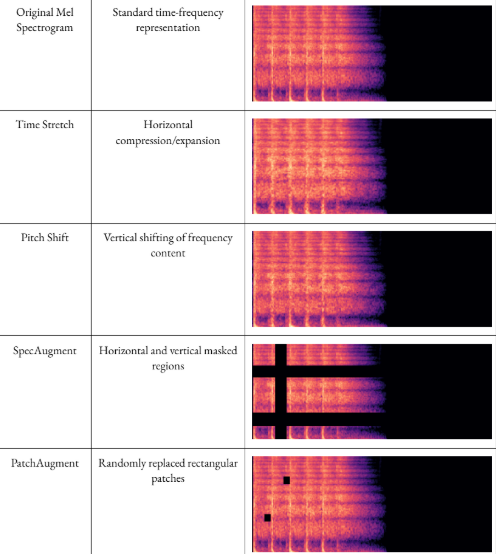
\includegraphics[width=1\linewidth]{latex//assets/augmentations.PNG}
    \caption{Spectrogram Augmentations Visualized}
    
\end{figure}
The final dataset assembled for our experimental work represents a substantial collection of urban sound data, meticulously organized for machine learning applications. It comprises approximately 58,000 spectrogram images distributed across 13 distinct classes. These classes include all original UrbanSound8K categories except for the general "siren" class, which was removed to avoid semantic overlap, plus four newly added vehicle classes that enhance the dataset's representation of urban transportation sounds.
Each audio sample was transformed into a standardized RGB image format (224x224 pixels) representing mel spectrograms. This uniform dimension ensures compatibility with common deep learning architectures, particularly convolutional neural networks that are frequently employed for image classification tasks. The dataset maintains the original 10-fold cross-validation structure, which is crucial for ensuring reliable and comparable performance evaluation across different models and studies.
\begin{table*}[ht]
  \centering
  \begin{tabular}{|p{3cm}|p{5cm}|}
    \hline
    \textbf{Parameter}& \textbf{Configuration}\\
    \hline
    FFT window size& 2048 samples\\
    \hline
    Hop length& 512 samples\\
    \hline
    Number of mel bands& 128\\
    \hline
    Frequency range& 20Hz to 8000Hz\\
    \hline
 Sample rate& 48kHz\\\hline
 Duration&4 seconds\\\hline
  \end{tabular}
  \caption{Mel-Spectrograms Parameter Configurations}
\end{table*}
\section{Methodology}
\subsection{Audio Representation}
For our research, we will represent audio data as spectrograms rather than raw waveforms, providing several advantages. Firstly, converting time-domain audio signals to frequency-domain spectrograms allows us to leverage powerful CNN architectures originally designed for image classification. Secondly, Mel spectrograms retain perceptually relevant features while reducing dimensionality.
We will use the following parameters for generating mel spectrograms as mentioned in Table 2.

\subsection{CNN Backbone Architectures}
\subsubsection{AlexNet}
AlexNet represents a pioneering CNN architecture that, while originally designed for image classification, has demonstrated considerable utility for audio event classification tasks. As a foundational deep learning model, AlexNet offers several characteristics that make it suitable for audio classification research. We believe that it provides a well-established baseline against which to measure the performance improvements of more modern architectures and its relatively lightweight nature makes it suitable for scenarios where computational resources are limited
\subsubsection{ResNet-18}
ResNet (Residual Network) architectures have proven highly effective for audio classification tasks due to their ability to mitigate the vanishing gradient problem through skip connections. These skip connections allow the network to learn residual functions, enabling the training of much deeper networks. We select the ResNet-18 variant which offers a good balance between performance and computational efficiency, making it suitable for real-time applications. Studies have shown that even this relatively shallow ResNet can achieve impressive results on audio classification tasks.
For audio event classification specifically, ResNet architectures have demonstrated strong performance in polyphonic sound event detection, with some implementations achieving F1-scores of 36.09\% on challenging DCASE datasets
\subsubsection{MobileNet}
MobileNetV2 represents an excellent choice for resource-constrained environments. This architecture is characterized by an inverted residual structure where residual connections are between bottleneck layers, lightweight depthwise convolutions for feature filtering, linear bottlenecks to preserve information flow. has been successfully implemented in real-time audio classification systems, demonstrating its practical utility. The architecture's efficiency makes it particularly suitable for edge computing applications, with some implementations requiring only 1 second of audio for accurate predictions.
\subsubsection{EfficientNet}
EfficientNet-B0 represents an innovative approach to model scaling that balances width, depth, and resolution. For audio classification tasks, it has demonstrated strong performance in heartbeat sound classification, achieving accuracy rates of 82\% when classifying Mel spectrograms of heart rate signals. In bird species audio identification, EfficientNet-B0 has been successfully employed as part of ensemble approaches, with researchers noting its balance of performance and computational efficiency. The compound scaling method used in EfficientNet makes it particularly effective at extracting features from spectrograms while maintaining reasonable computational requirements. EfficientNet-B0 serves as the baseline model in this family, providing a good starting point for audio classification tasks before considering larger variants if needed.
\subsubsection{ConvNeXt}
ConvNeXt represents one of the most recent advancements in CNN architecture design, incorporating lessons learned from transformer models while maintaining the inductive biases of CNNs. ConvNeXt-Tiny has shown remarkable performance in audio classification tasks. It achieved a mean average precision (mAP) of 0.471 on AudioSet, which is comparable to or better than much larger transformer-based models while using significantly fewer parameters. The architecture has been successfully adapted for audio tagging tasks, demonstrating its versatility across different audio classification scenarios. ConvNeXt-Tiny's performance is particularly impressive considering it uses only about 28 million parameters, making it much more efficient than many transformer-based alternatives.
\subsubsection{Inception/VGG}
Including Inception v3 and VGG16 as baseline comparisons is methodologically sound since Inception v3 has been successfully applied to audio classification using transfer learning. It has shown good results in broadcast audio classification tasks, achieving accuracy rates of 94\% when classifying TV broadcast audio into categories like advertisements, cartoons, news, songs, and sports. VGG16 serves as a useful baseline due to its straightforward architecture. While newer models often outperform it, VGG's simple design makes it valuable for comparative analysis and establishing performance floors
Our k-fold cross-validation framework will systematically evaluate these architectures using the following metrics: Classification accuracy, F1-score (particularly for imbalanced classes), Confusion matrix analysis and GradCAM visualizations for model interpretability.

\subsection{Self-Supervised Learning Techniques}
\subsubsection{SimCLR}
SimCLR represents one of the most influential contrastive learning frameworks, and its adaptation to audio spectrograms shows considerable promise. When applied to spectrograms, SimCLR requires audio-appropriate augmentations such as time masking, frequency masking, and time shifting rather than the traditional image-based augmentations. Its performance on audio data is highly dependent on the augmentation strategy. Studies indicate that combinations of time and frequency masking are particularly effective for spectrogram-based learning. The large batch sizes typically required by SimCLR (4096+ in original implementation) can be challenging for audio processing, though recent modifications have shown effective performance with smaller batches (256-512) when using specialized optimization techniques.
\subsubsection{MoCo}
MoCo's queue-based approach offers several advantages when applied to audio spectrograms. The queue mechanism allows for a large number of negative samples without requiring extremely large batch sizes, making it particularly suitable for high-resolution audio spectrograms that may be memory-intensive. For audio spectrograms, MoCo implementations typically benefit from specialized convolutional architectures that account for the time-frequency structure of spectrograms.
\subsubsection{BYOL}
BYOL's negative-free approach offers unique advantages for audio data. Without relying on negative samples, BYOL has demonstrated superior performance on audio datasets with high intra-class variability, such as urban sound classification tasks. For audio spectrograms, BYOL's performance is highly dependent on the augmentation strategy. Research indicates that combining strong and weak augmentations (e.g., heavy time masking paired with light pitch shifting) produces optimal results. When applied to audio data, BYOL typically requires fewer training epochs to converge compared to contrastive methods like SimCLR, with studies showing strong performance after just 100-200 epochs versus 500+ for contrastive approaches.
\subsection{Non-Contrastive Methods}
\subsubsection{Barlow Twins}
Barlow Twins' redundancy reduction approach offers several benefits for audio representation learning. The cross-correlation objective naturally promotes disentangled representations of audio features, which has proven particularly effective for separating overlapping sound events. Barlow Twins typically requires smaller batch sizes than contrastive methods, making it more practical for high-resolution audio spectrograms
\subsubsection{DINO}
DINO's self-distillation approach offers unique advantages for audio event classification. When applied to audio spectrograms, DINO has demonstrated superior ability to learn semantically meaningful features that correspond to distinct audio events, even without explicit supervision. The self-attention components in DINO are particularly effective at capturing long-range dependencies in audio, which is crucial for identifying events that span extended time periods. For audio spectrograms, DINO benefits from multi-scale approaches that can capture both fine-grained spectral details and broader temporal patterns.
\subsubsection{SwAV}
SwAV's clustering-based approach offers several advantages for audio event classification. The online clustering approach naturally groups similar audio events, creating prototype representations that correspond to meaningful audio categories. SwAV's simultaneous clustering and representation learning is particularly efficient for audio data, requiring fewer computational resources than traditional contrastive approaches. Its swapped prediction mechanism ensures consistency across different views of the same audio segment, which is particularly valuable for handling variations in audio recordings.
\subsection{Data Augmentation Strategies}
We employ the following specialized data augmentation techniques for audio spectrograms:
1. Time Stretching: Modification of audio playback speed without affecting pitch.
   - Implementation: librosa's time\_stretch with rates of 0.8x and 1.2x
   - Effect: Increases robustness to tempo variations
2. Pitch Shifting: Altering the pitch while maintaining tempo.
   - Implementation: librosa's pitch\_shift with ±2 semitones
   - Effect: Improves generalization across pitch variation
3. SpecAugment: Applying time and frequency masking to spectrograms.
   - Implementation: Random masking of time and frequency bands (2 masks each, max width 20)
   - Effect: Improves robustness to missing frequency components and temporal variations
4. PatchAugment: Randomly replacing patches in spectrograms.
   - Implementation: Random replacement of 5 patches of size 10x10
   - Effect: Enhances model's ability to focus on global spectral patterns
5. Noise Addition: Adding controlled Gaussian noise.
   - Implementation: Addition of noise at different SNR levels (5dB and 15dB)
   - Effect: Improves performance in noisy environments
\subsection{Training  \& Evaluation Methodology}
\begin{figure*}[t]
  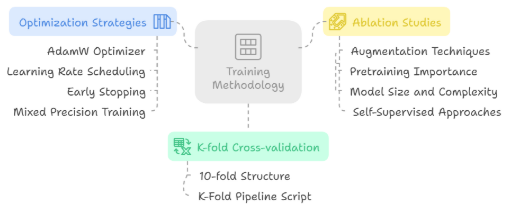
\includegraphics[width=0.48\linewidth]{latex/assets/training_framework.PNG} \hfill
  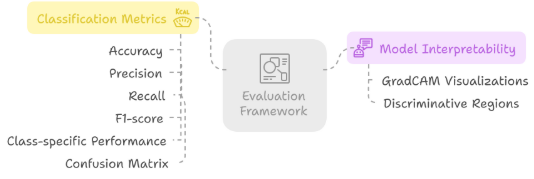
\includegraphics[width=0.48\linewidth]{latex/assets/evaluation_framework.PNG}
  \caption {Training and Evaluation Framework for QUACLRS}
\end{figure*}
The training methodology for our audio event classification system employs a comprehensive K-fold cross-validation approach to ensure robust model evaluation and generalization. This section details the key components of our training pipeline, highlighting implementation choices and their rationale. We implement a 10-fold cross-validation strategy to maximize the reliability of our model evaluation. For each fold:
\begin{itemize}
    \item The dataset is partitioned into 10 equal segments
    \item Each fold serves as a test set exactly once
    \item The preceding fold (wrapping around if needed) serves as the validation set
    \item The remaining 8 folds constitute the training set
\end{itemize}
This approach ensures that every sample appears exactly once in the test set across all folds, the validation set remains distinct from both training and test sets, and the maximum amount of data is available for training while maintaining separate validation and test sets.
Our training pipeline supports multiple CNN architectures with flexible configuration options. The model initialization process includes architecture selection from a range of modern CNN models (AlexNet, VGG16, ResNet18, MobileNet, Inception, EfficientNet, and ConvNeXt), optional transfer learning through pretrained weights and selective feature freezing for efficient fine-tuning. To address the common challenge of class imbalance in audio event classification, we implement a weighted loss function approach. Class weights are calculated inversely proportional to class frequencies in the training set and applied to the CrossEntropyLoss function. This ensures that minority classes receive higher importance during training, preventing the model from being biased toward majority classes. 
Our optimization approach combines adaptive learning rate methods with regularization techniques. We use Adam optimizer with configurable learning rate and weight decay parameters and provide two learning rate scheduling options: ReduceLROnPlateau which reduces learning rate when validation accuracy plateaus and CosineAnnealingLR, which gradually reduces learning rate following a cosine curve.
To prevent overfitting and ensure efficient training, we implement an early stopping mechanism that monitors validation accuracy. raining continues until no improvement is seen for a predefined number of epochs (patience), the best model based on validation accuracy is saved and the training terminates when the patience threshold is exceeded. To improve training efficiency on modern GPUs, we implement automatic mixed precision training using PyTorch's GradScaler. This technique performs forward and backward passes using lower precision (FP16) where appropriate while maintaining a master copy of weights in full precision (FP32). It uses a gradient scaler to prevent underflow and accelerates training on compatible hardware significantly.
Finally, our evaluation protocol includes multiple metrics and visualization techniques to provide a thorough assessment of model performance.
\begin{itemize}
    \item Standard metrics: accuracy, precision, recall, F1-score
    \item Confusion matrix visualization
    \item ROC curves for multi-class classification
    \item Grad-CAM visualizations for model interpretability
\end{itemize}
Our methodology also includes systematic aggregation of results across all folds where the average performance metrics are calculated across all folds, individual fold performances are recorded, and all training parameters and configurations are saved with the experiments timestamped for reproducibility.
\section{Results}
\subsection{CNN Backbones}
\begin{figure*}[ht]
    \centering
    % First row with 4 matrices
    \begin{subfigure}[b]{0.24\textwidth}
        \centering
        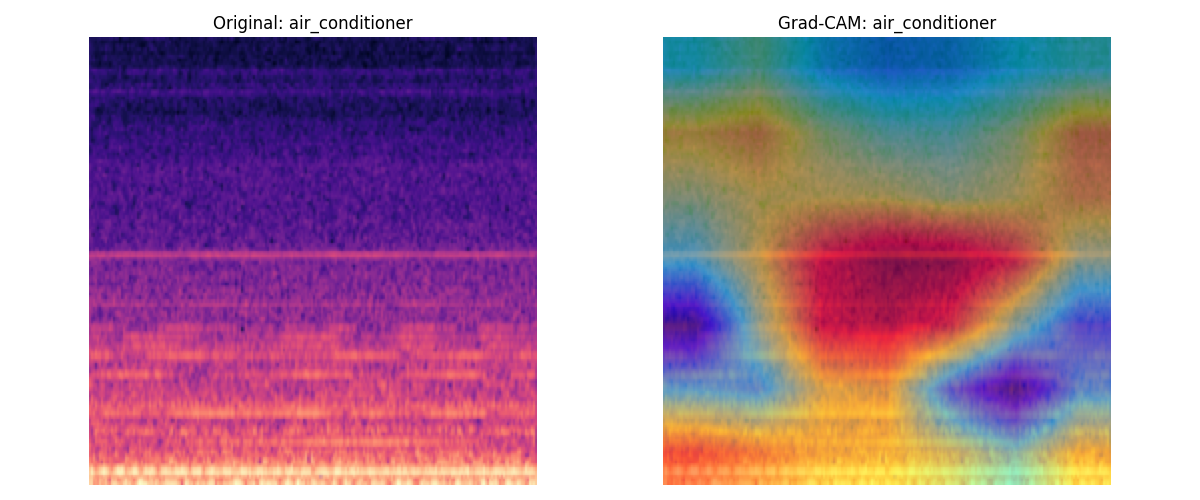
\includegraphics[width=\textwidth]{latex/assets/efficientnet_fold7_gradcam/gradcam_air_conditioner_0.png}
        \caption{Air Conditioner}
    \end{subfigure}
    \hfill
    \begin{subfigure}[b]{0.24\textwidth}
        \centering
        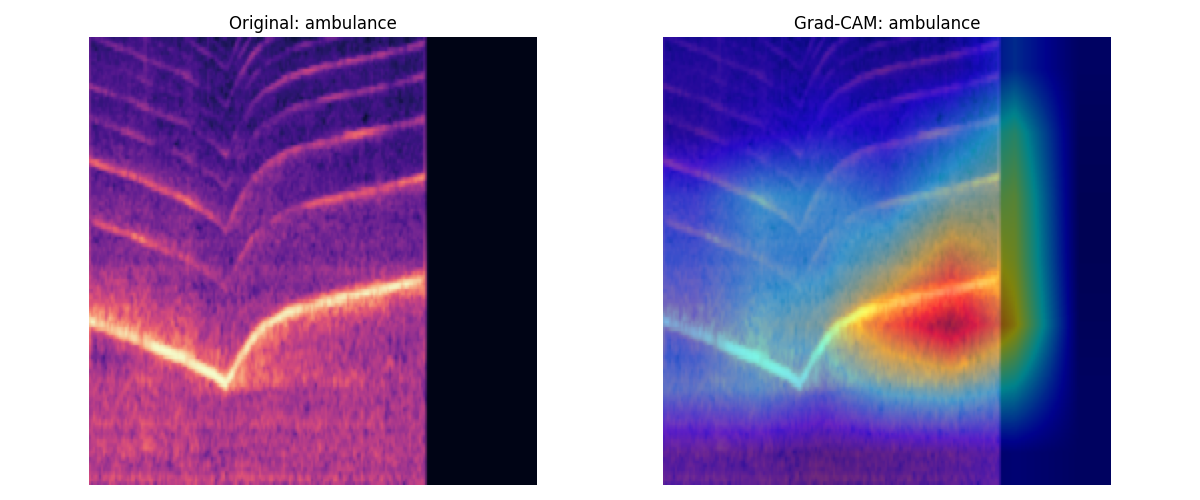
\includegraphics[width=\textwidth]{latex/assets/efficientnet_fold7_gradcam/gradcam_ambulance_0.png}
        \caption{Ambulance}
    \end{subfigure}
    \hfill
    \begin{subfigure}[b]{0.24\textwidth}
        \centering
        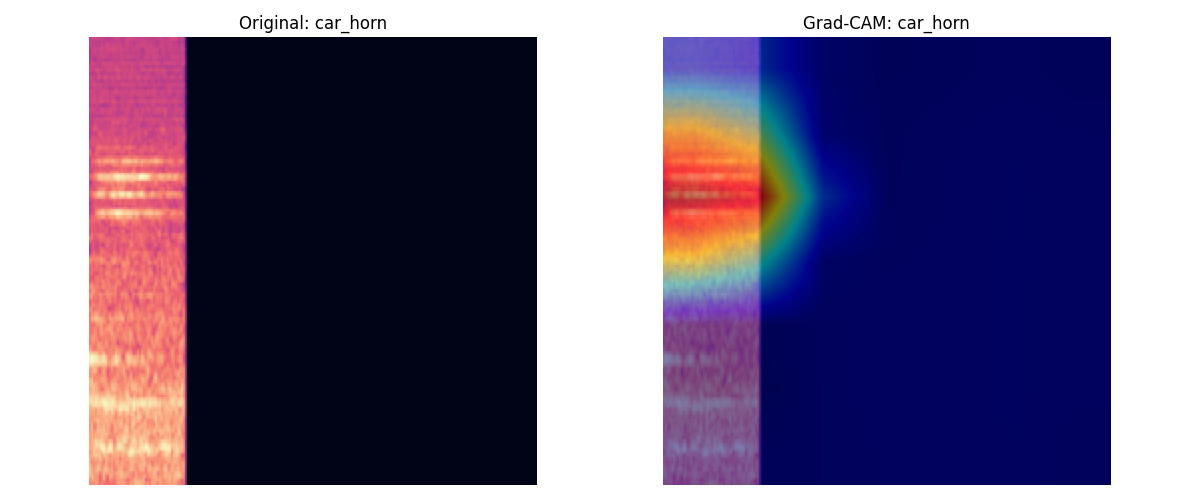
\includegraphics[width=\textwidth]{latex/assets/efficientnet_fold7_gradcam/gradcam_car_horn_0.png}
        \caption{Car Horn}
    \end{subfigure}
    \hfill
    \begin{subfigure}[b]{0.24\textwidth}
        \centering
        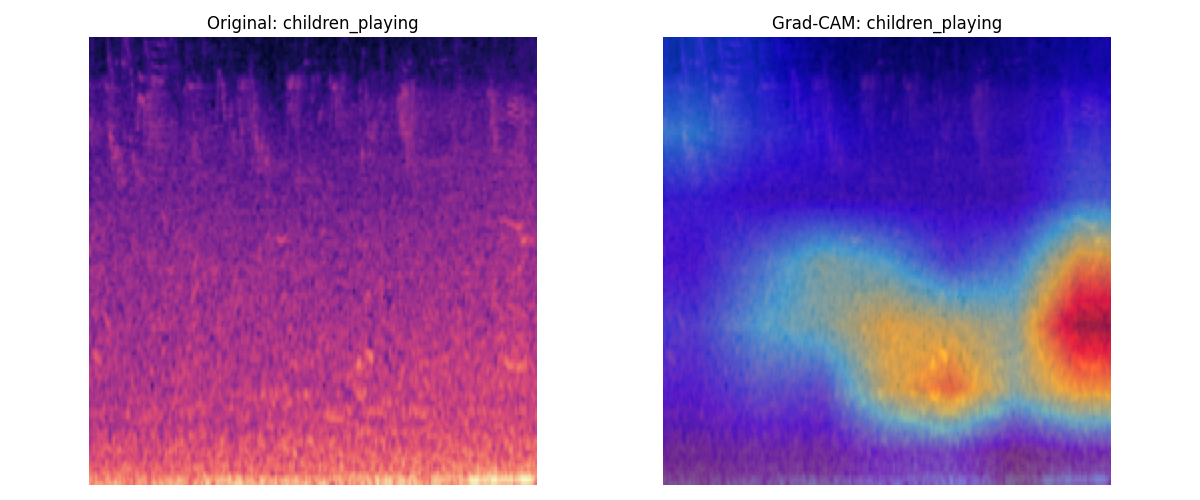
\includegraphics[width=\textwidth]{latex/assets/efficientnet_fold7_gradcam/gradcam_children_playing_0.png}
        \caption{Children Playing}
    \end{subfigure}
    
    \vspace{0.5cm}
    
    % Second row with 3 matrices (centered)
    \begin{subfigure}[b]{0.24\textwidth}
        \centering
        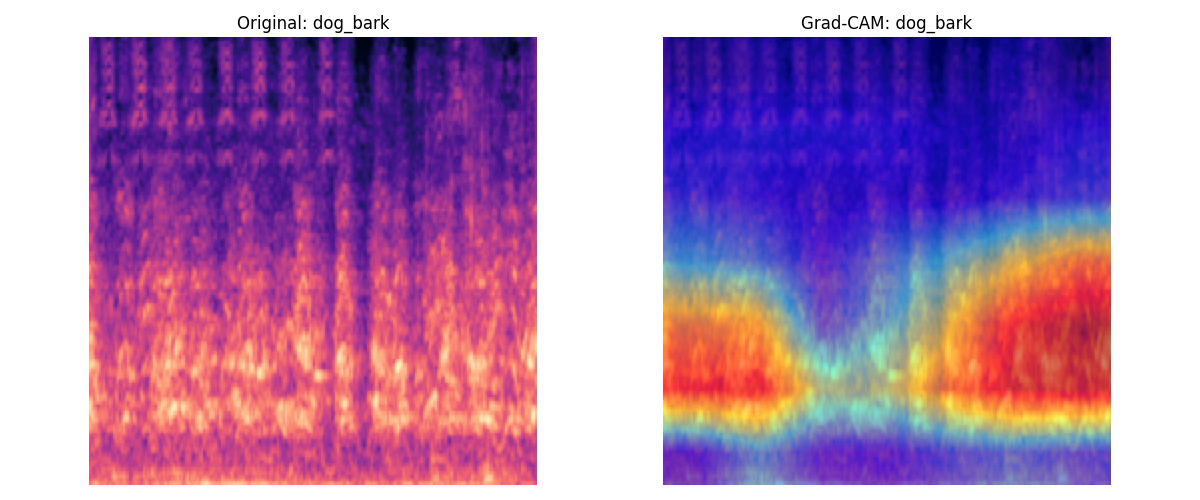
\includegraphics[width=\textwidth]{latex/assets/efficientnet_fold7_gradcam/gradcam_dog_bark_0.png}
        \caption{Dog Barking}
    \end{subfigure}
    \hfill
    \begin{subfigure}[b]{0.24\textwidth}
        \centering
        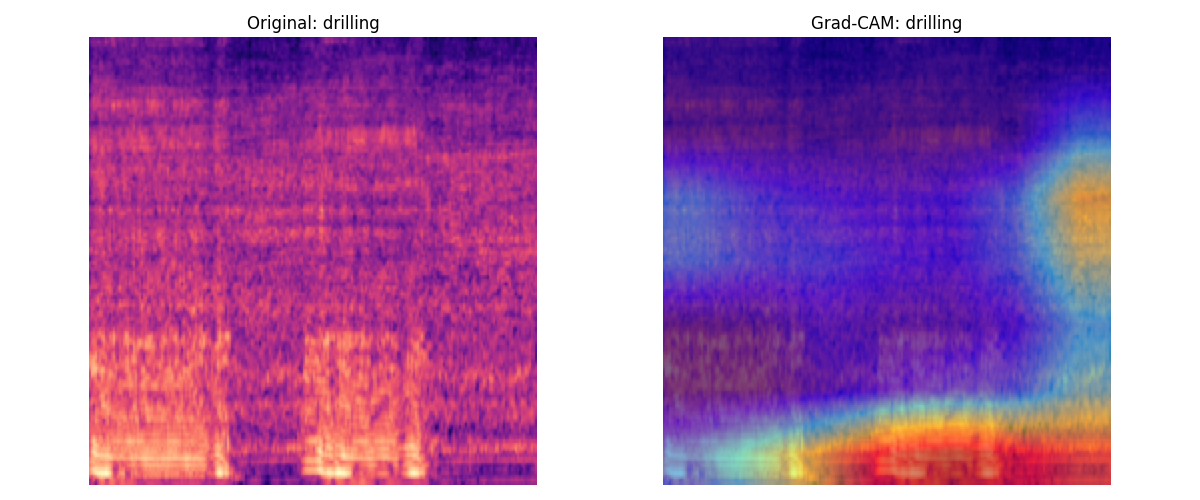
\includegraphics[width=\textwidth]{latex/assets/efficientnet_fold7_gradcam/gradcam_drilling_0.png}
        \caption{Drilling}
    \end{subfigure}
    \hfill
    \begin{subfigure}[b]{0.24\textwidth}
        \centering
        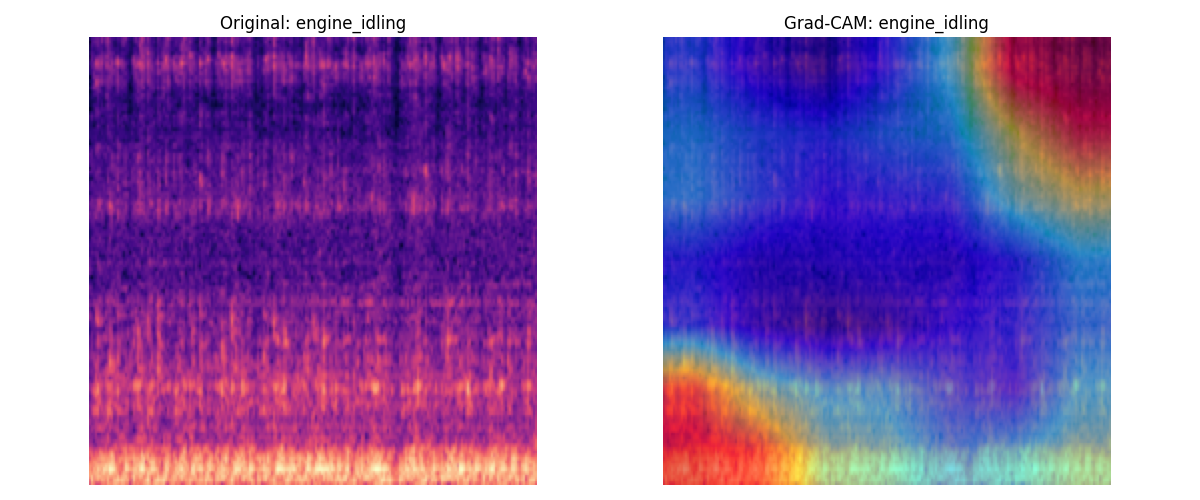
\includegraphics[width=\textwidth]{latex/assets/efficientnet_fold7_gradcam/gradcam_engine_idling_0.png}
        \caption{Engine Idling}
    \end{subfigure}
    \hfill
    \begin{subfigure}[b]{0.24\textwidth}
        \centering
        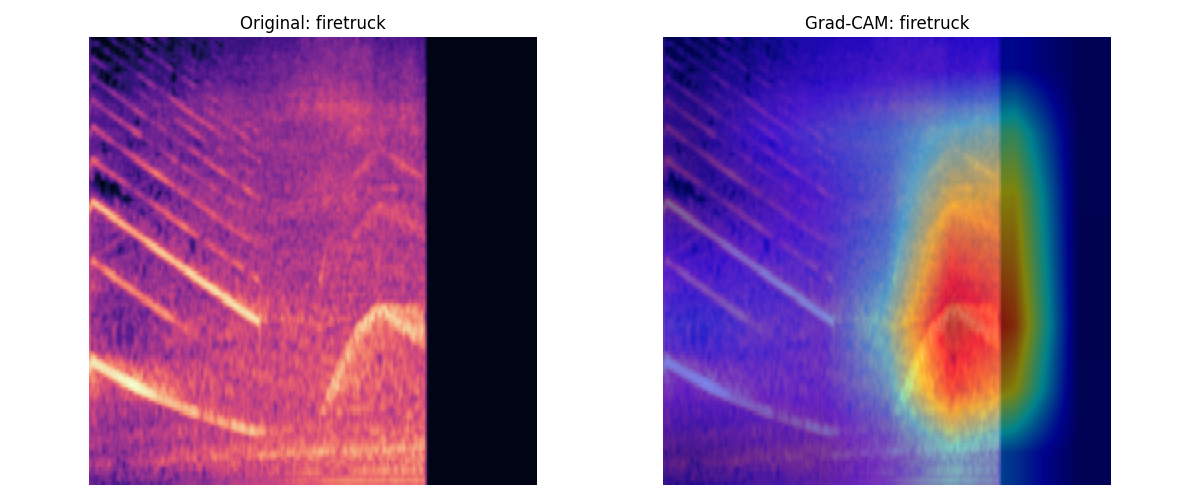
\includegraphics[width=\textwidth]{latex/assets/efficientnet_fold7_gradcam/gradcam_firetruck_0.png}
        \caption{Firetruck}
    \end{subfigure}
    \hfill
    \begin{subfigure}[b]{0.24\textwidth}
        \centering
        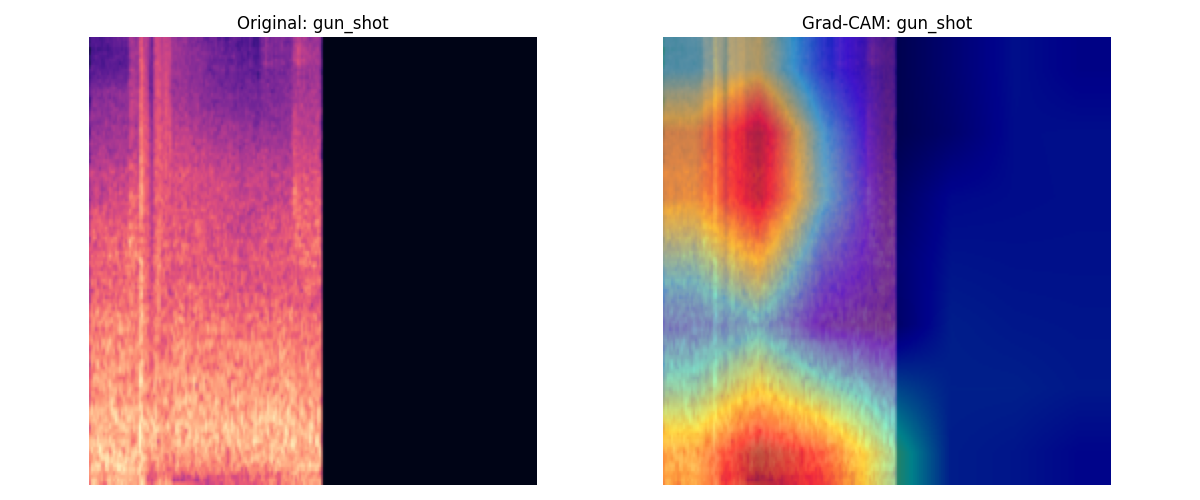
\includegraphics[width=\textwidth]{latex/assets/efficientnet_fold7_gradcam/gradcam_gun_shot_0.png}
        \caption{Gun Shot}
    \end{subfigure}
    \hfill
    \begin{subfigure}[b]{0.24\textwidth}
        \centering
        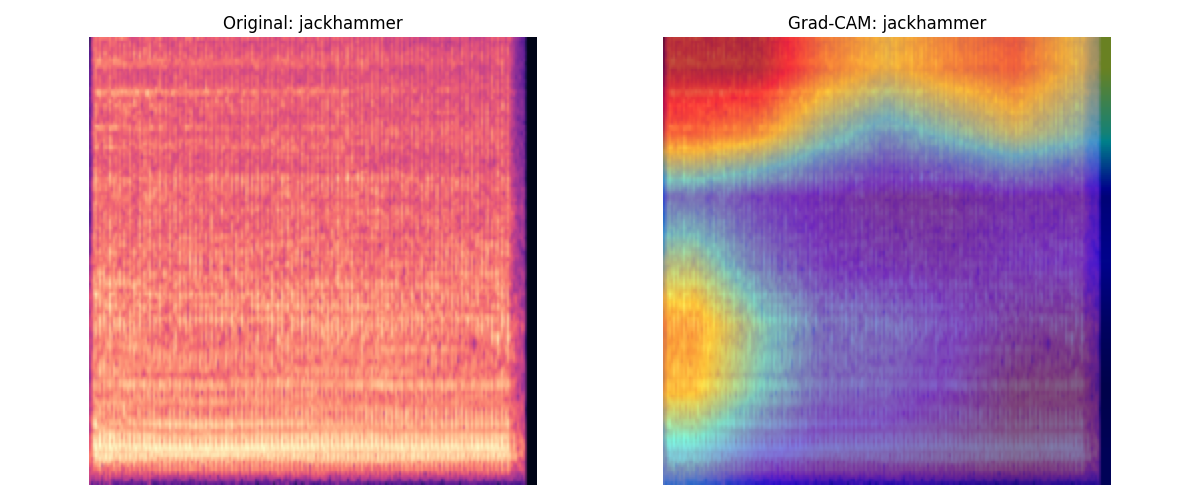
\includegraphics[width=\textwidth]{latex/assets/efficientnet_fold7_gradcam/gradcam_jackhammer_0.png}
        \caption{Jackhammer}
    \end{subfigure}
    \hfill
    \begin{subfigure}[b]{0.24\textwidth}
        \centering
        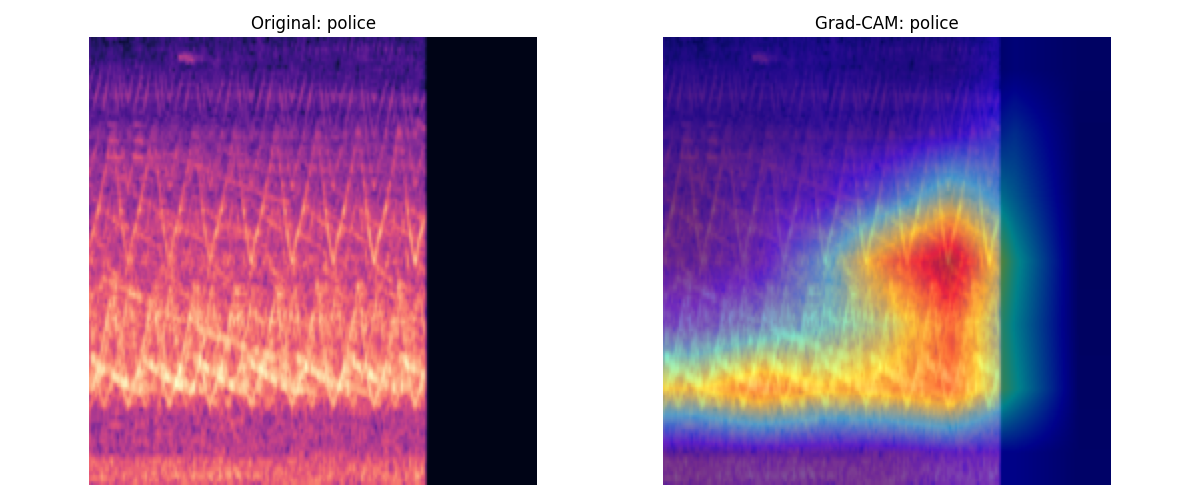
\includegraphics[width=\textwidth]{latex/assets/efficientnet_fold7_gradcam/gradcam_police_0.png}
        \caption{Police}
    \end{subfigure}
    \hfill
    \begin{subfigure}[b]{0.24\textwidth}
        \centering
        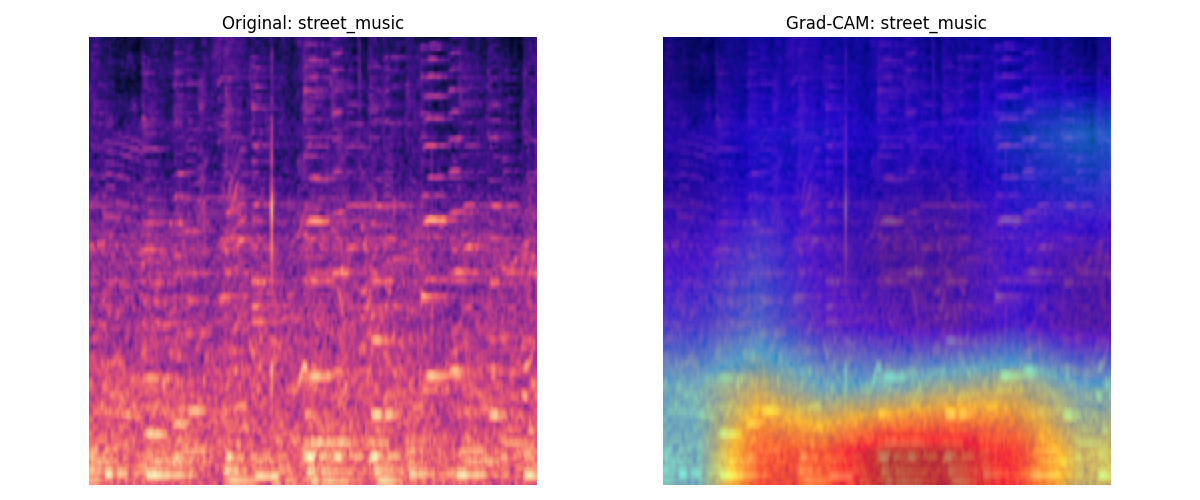
\includegraphics[width=\textwidth]{latex/assets/efficientnet_fold7_gradcam/gradcam_street_music_0.png}
        \caption{Street Music}
    \end{subfigure}
    \hfill
    \begin{subfigure}[b]{0.24\textwidth}
        \centering
        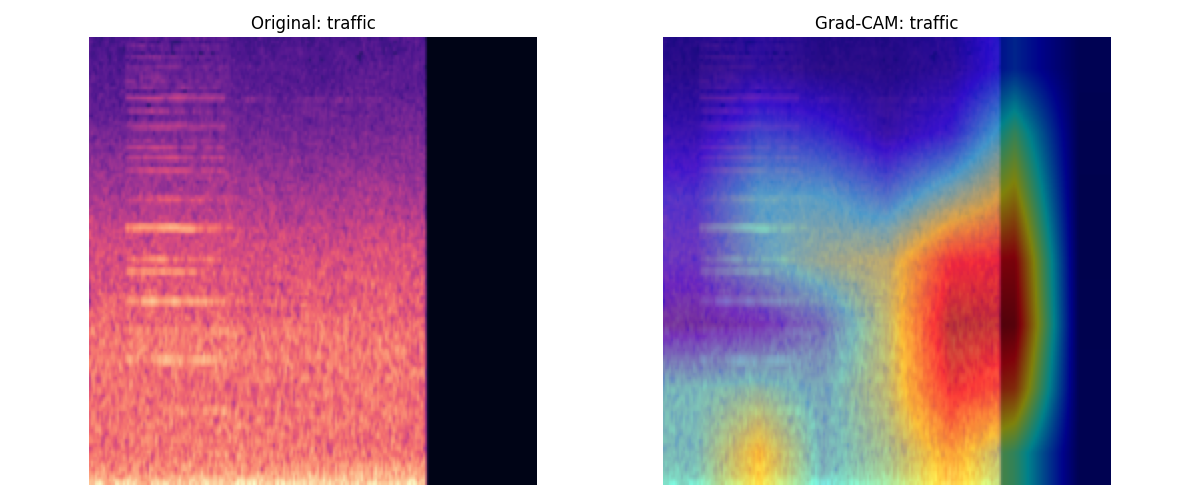
\includegraphics[width=\textwidth]{latex/assets/efficientnet_fold7_gradcam/gradcam_traffic_0.png}
        \caption{Traffic}
    \end{subfigure}
    
    \caption{GradCam Visualizations for EfficientNet Pre-trained Fold 7 Trained Results}
\end{figure*}
\begin{figure*}[ht]
    \centering
    % First row with 4 matrices
    \begin{subfigure}[b]{0.24\textwidth}
        \centering
        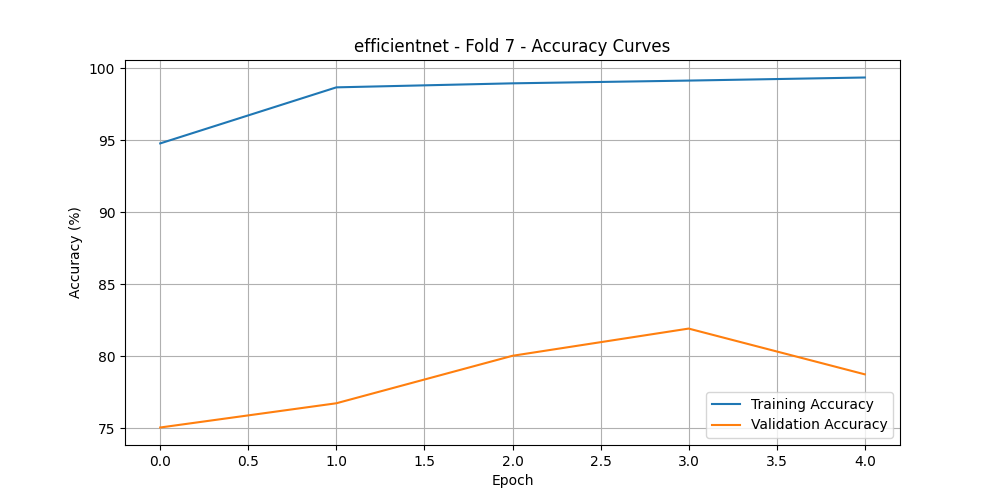
\includegraphics[width=\textwidth]{latex/assets/efficientnet_pretrained_fold7/accuracy_curves.png}
        \caption{Accuracy Curves}
    \end{subfigure}
    \hfill
    \begin{subfigure}[b]{0.24\textwidth}
        \centering
        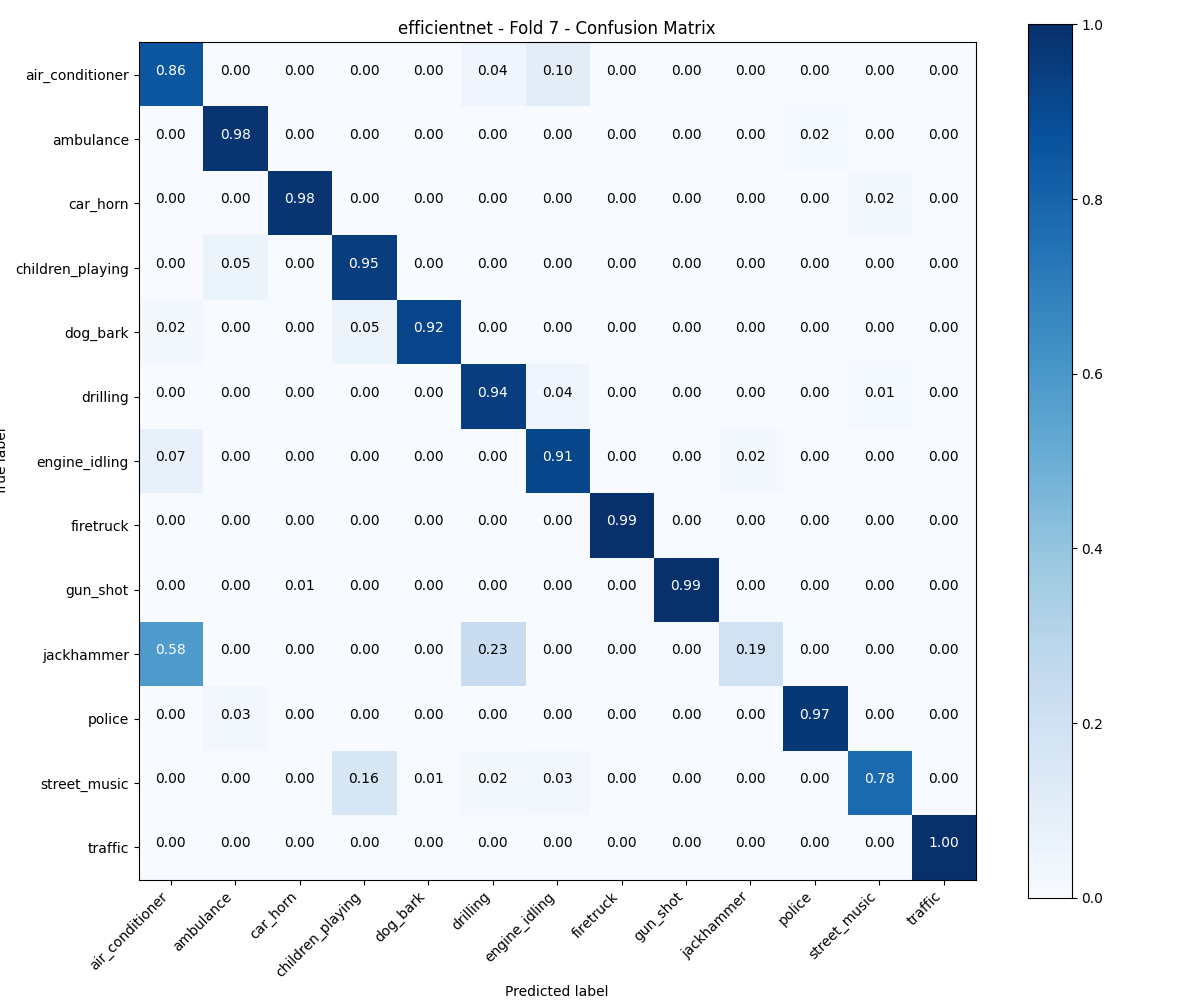
\includegraphics[width=\textwidth]{latex/assets/efficientnet_pretrained_fold7/confusion_matrix.png}
        \caption{Confusion Matrix}
    \end{subfigure}
    \hfill
    \begin{subfigure}[b]{0.24\textwidth}
        \centering
        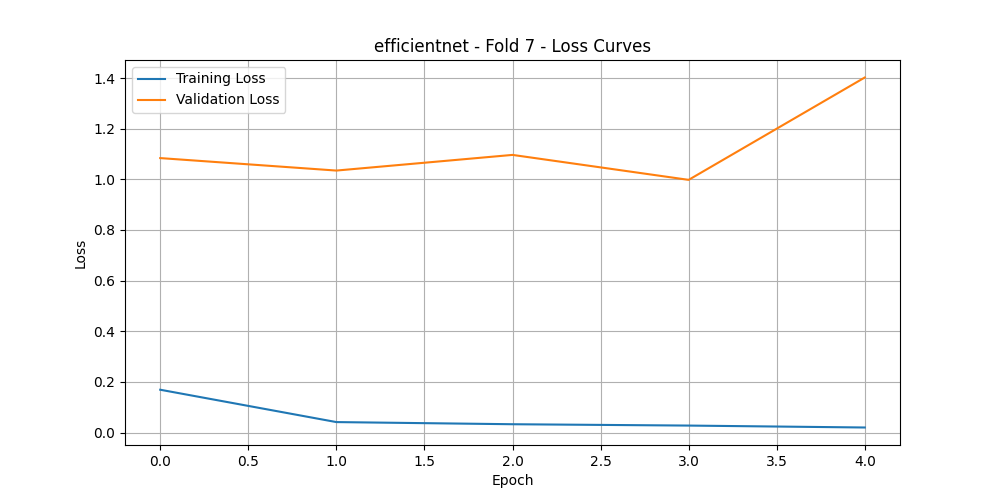
\includegraphics[width=\textwidth]{latex/assets/efficientnet_pretrained_fold7/loss_curves.png}
        \caption{Loss Curves}
    \end{subfigure}
    \hfill
    \begin{subfigure}[b]{0.24\textwidth}
        \centering
        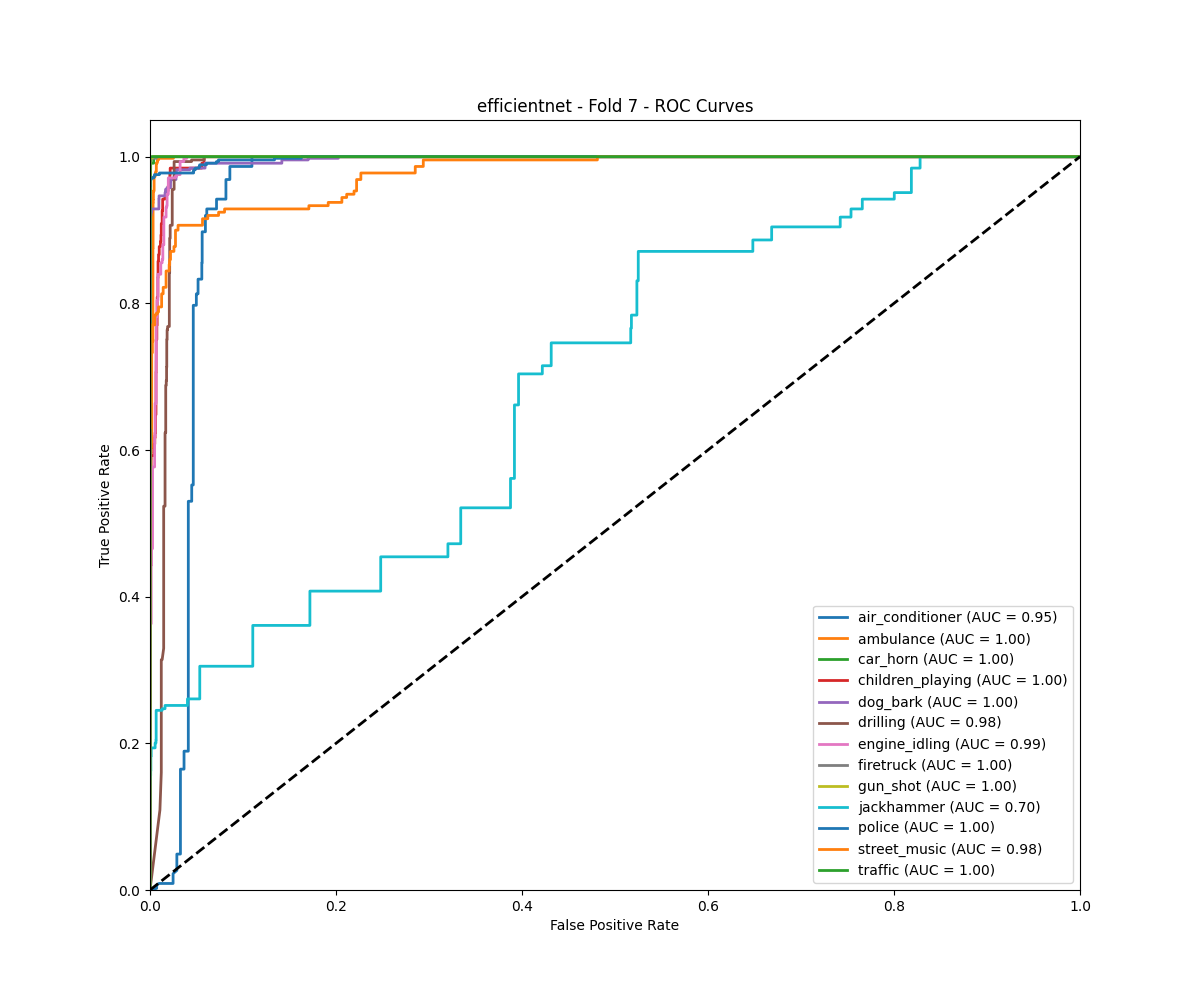
\includegraphics[width=\textwidth]{latex/assets/efficientnet_pretrained_fold7/roc_curves.png}
        \caption{ROC Curves}
    \end{subfigure}
    \caption{Accuracy Curves, Confusion Matrix, Loss Curves and ROC Curves Visualizations (in that order) for EfficientNet Pre-trained Backbone on Trained on Fold 7}
\end{figure*}
\begin{table*}[ht]
    \centering
    \begin{tabular}{|l|c|c|c|l|} \hline  
         \textbf{Architecture}& \textbf{Average Accuracy}& \textbf{Performance Rank}&\textbf{Accuracy Range} &\textbf{Std. Deviation}\\ \hline  
         
         EfficientNet& 82.09\%& 1&79.02\% - 88.30\%&3.36\%\\ \hline  
         Inception& 80.91\%& 2&74.50\% - 86.48\%&4.40\%\\ \hline  
         MobileNet& 80.60\%& 3&76.89\% - 85.79\%&2.86\%\\ \hline
         ResNet18& 79.33\%& 4&74.76\% - 83.82\%&2.94\%\\\hline
         ConvNext& 79.18\%& 5&74.20\% - 88.13\%&4.13\%\\\hline
         AlexNet& 73.40\%& 6&67.80\% - 79.79\%&4.14\%\\\hline
         VGG16& 65.73\%& 7&60.36\% - 71.21\%&3.53\%\\\hline  
    \end{tabular}
    \caption{Performance Comparison of CNN Architectures: 10 Fold 5 Epoch} 
\end{table*}
We discuss the results for the 10 Fold, 5 Epoch Training of 7 CNN Algorithms as part of our study using pretrained weights in this section, the remaining shall be covered in our ablation section. 
EfficientNet emerges as the top performer in our audio event classification study, achieving an impressive 82.09\% average accuracy across 10-fold cross-validation. Its compound scaling approach, which systematically balances network depth, width, and resolution, delivers exceptional results with remarkable consistency. The architecture maintains stable performance across most folds (79-81\% accuracy), while achieving peak performance of 88.30\% in fold 7 and 88.22\% in fold 9. This stability across different data splits demonstrates strong generalization capabilities, making it particularly suitable for audio classification tasks. These findings align with recent research from the BirdCLEF 2024 challenge, where EfficientNet models (specifically B0 and B1 variants) proved highly effective for bird species audio identification, with researchers noting its balance of performance and computational efficiency.
The Inception architecture ranks second with an 80.91\% average accuracy, though with notably higher variability (74.50\% to 86.48\%) than EfficientNet. Its multi-scale feature extraction approach, using parallel convolutional filters of varying sizes, effectively captures diverse acoustic patterns. However, the 12\% performance gap between best and worst folds suggests potential sensitivity to data distribution variations. This architecture's strong performance aligns with previous findings in broadcast audio classification tasks, where Inception v3 has demonstrated accuracy rates of 94\% when classifying TV broadcast audio into categories like advertisements, cartoons, news, songs, and sports.
MobileNet achieves a competitive 80.60\% average accuracy, demonstrating an excellent balance between performance and computational efficiency. Its depthwise separable convolutions deliver consistent mid-range performance (77-82\% across most folds), with two folds exceeding 85\% accuracy. This architecture's combination of strong performance and low computational requirements makes it particularly suitable for deployment in resource-constrained environments. These findings are consistent with research on YAMNet (Yet Another Audio MobileNet), a pre-trained deep neural network model for audio event classification developed by Google that utilizes the MobileNet architecture and has been specifically designed for mobile and embedded applications with a focus on low latency.
Finally, ResNet18 and ConvNext show similar average performance (79.33\% and 79.18\% respectively), though ConvNext exhibits higher variability and the highest individual fold result (88.13\%). AlexNet achieves a respectable 73.40\% despite its relative simplicity, while VGG16 lags significantly at 65.73\%. The substantial performance gap between AlexNet and VGG16 aligns with previous research in voice identification tasks, where AlexNet achieved approximately 65.95\% accuracy compared to ResNet's 97.2\% on the same dataset. Despite VGG16's popularity in image classification, its uniform filter size and simple stacking approach appear less effective for audio classification tasks compared to more modern architectures with specialized design elements.
\subsection{SSL Methods}
\begin{table*}[ht]
    \centering
    \begin{tabular}{|l|c|c|c|} \hline  
         \textbf{Algorithm}& \textbf{Accuracy}& \textbf{Macro Avg F1}&\textbf{Weighted Avg F1}\\ \hline  
         
         SimCLR& 65.00\%& 0.64 &0.66\\ \hline  
         MoCo V2& 62.00\% & 0.62&0.59\\ \hline  
         MoCo& 60.00\% & 0.59&0.61\\ \hline
         BYOL& 46.00\% & 0.40&0.41\\\hline
         SwAV& 39.00\%& 0.33&0.34\\\hline
         DINO& 27.00\% & 0.24&0.26\\\hline
         Barlow Twins& 8.00\% & 0.09&0.07\\\hline  
    \end{tabular}
    \caption{Overall Performance Comparison for 1-Fold-1-Epoch Evaluation of SSL Algorithms using Resnet-18 Backbone}
\end{table*}
\begin{table*}[ht]
    \centering
    \small
    \begin{tabular}{l|ccccccc}
    \hline
    \textbf{Sound Class} & \textbf{SimCLR} & \textbf{MoCoV2} & \textbf{MoCo} & \textbf{BYOL} & \textbf{SwAV} & \textbf{DINO} & \textbf{BarlowTwins} \\
    \hline
    air\_conditioner  & 0.51 & 0.69 & 0.78 & 0.28 & 0.00 & 0.32 & 0.00 \\
    ambulance        & 0.81 & 0.91 & 0.74 & 0.47 & 0.43 & 0.18 & 0.00 \\
    car\_horn         & 0.33 & 0.05 & 0.35 & 0.54 & 0.05 & 0.00 & 0.00 \\
    children\_playing & 0.89 & 0.83 & 0.69 & 0.67 & 0.00 & 0.24 & 0.00 \\
    dog\_bark         & 0.69 & 0.82 & 0.71 & 0.62 & 0.55 & 0.66 & 0.25 \\
    drilling         & 0.61 & 0.64 & 0.42 & 0.00 & 0.30 & 0.15 & 0.00 \\
    engine\_idling    & 0.45 & 0.30 & 0.42 & 0.02 & 0.34 & 0.17 & 0.00 \\
    firetruck        & 0.68 & 0.82 & 0.56 & 0.40 & 0.40 & 0.42 & 0.22 \\
    gun\_shot         & 0.26 & 0.51 & 0.38 & 0.43 & 0.27 & 0.34 & 0.03 \\
    jackhammer       & 0.74 & 0.00 & 0.88 & 0.65 & 0.71 & 0.31 & 0.01 \\
    police           & 0.81 & 0.95 & 0.62 & 0.04 & 0.17 & 0.00 & 0.40 \\
    street\_music     & 0.71 & 0.72 & 0.32 & 0.67 & 0.46 & 0.11 & 0.08 \\
    traffic          & 0.88 & 0.84 & 0.86 & 0.38 & 0.58 & 0.20 & 0.14 \\
    \hline
    \end{tabular}
    \caption{F1-scores for different sound classes across SSL algorithms}
\end{table*}


In this section, we analyze the performance of seven self-supervised learning (SSL) algorithms on audio classification tasks. The evaluation was conducted using a 1-fold validation approach with a single epoch of training. Table 1 summarizes the key performance metrics for each algorithm.
SimCLR demonstrates the strongest overall performance among the evaluated SSL algorithms, achieving 65\% accuracy and a weighted F1-score of 0.66. This algorithm shows particularly robust performance across a diverse range of sound classes:
\begin{itemize}
    \item Excellent performance on "children\_playing" (F1: 0.89), "traffic" (F1: 0.88), and "police" (F1: 0.81)
    \item Strong performance on "ambulance" (F1: 0.81) and "jackhammer" (F1: 0.74)
    \item Moderate effectiveness on "street\_music" (F1: 0.71) and "dog\_bark" (F1: 0.69)
    \item Weaker performance on "gun\_shot" (F1: 0.26) and "car\_horn" (F1: 0.33)
\end{itemize}
The balanced precision and recall across most classes suggest it learns representations that effectively capture the distinctive characteristics of various sound types. Its superior performance can be attributed to its contrastive learning approach that effectively distinguishes between different audio signals in the embedding space.
MoCoV2 achieves the second-best performance with 62\% accuracy. We notice:
\begin{itemize}
    \item Excellent performance on "police" (F1: 0.95), "ambulance" (F1: 0.91), and "traffic" (F1: 0.84)
    \item Strong performance on "children\_playing" (F1: 0.83) and "dog\_bark" (F1: 0.82)
    \item MoCoV2 completely fails to classify "jackhammer" sounds (F1: 0.00)
    \item Low performance on "car\_horn" (F1: 0.05)
\end{itemize}
MoCoV2 shows more variability in class-wise performance compared to SimCLR, with several classes showing excellent results while others receive poor recognition. This suggests potential overfitting to certain sound characteristics.
The original MoCo algorithm achieves 60\% accuracy and a weighted F1-score of 0.61, showing:
\begin{itemize}
    \item Excellent performance on "jackhammer" (F1: 0.88) and "traffic" (F1: 0.86)
    \item Strong performance on "air\_conditioner" (F1: 0.78) and "ambulance" (F1: 0.74)
    \item More balanced performance across classes compared to MoCoV2
    \item Lowest performance on "car\_horn" (F1: 0.35) and "street\_music" (F1: 0.32)
\end{itemize}
MoCo demonstrates more consistent performance across classes compared to its successor MoCoV2, though with slightly lower overall accuracy. This suggests MoCo's momentum contrast approach effectively captures general audio features.
BYOL shows moderate performance with 46\% accuracy and a weighted F1-score of 0.41.
\begin{itemize}
    \item Strongest performance on "jackhammer" (F1: 0.65), "children\_playing" (F1: 0.67), and "street\_music" (F1: 0.67)
    \item Very poor performance on "drilling" (F1: 0.00) and "police" (F1: 0.04)
    \item Significant imbalance between precision and recall for many classes
\end{itemize}
BYOL's bootstrap your own latent (BYOL) approach, which doesn't rely on negative pairs, appears less effective for audio classification compared to contrastive methods like SimCLR and MoCo.
SwAV achieves 39\% accuracy with a weighted F1-score of 0.34:
\begin{itemize}
    \item Best performance on "jackhammer" (F1: 0.71) and "traffic" (F1: 0.58)
    \item Complete failure on "air\_conditioner" and "children\_playing" (F1: 0.00)
    \item Generally low precision across most classes
\end{itemize}
SwAV's clustering-based approach appears less effective for audio classification tasks compared to contrastive learning methods
DINO shows relatively weak performance with 27\% accuracy and a weighted F1-score of 0.26.
\begin{itemize}
    \item Strongest performance on "dog\_bark" (F1: 0.66)
    \item Several classes show perfect precision but very low recall (e.g., "jackhammer", "street\_music")
    \item Complete failure on "car\_horn" and "police" (F1: 0.00)
\end{itemize}
DINO's self-distillation approach with no labels seems to struggle with the complexity and variability of audio data.
BarlowTwins performs poorly with only 8\% accuracy and a weighted F1-score of 0.07.
\begin{itemize}
    \item Fails completely on 9 out of 13 classes (F1: 0.00)
    \item Best performance on "dog\_bark" (F1: 0.25) and "firetruck" (F1: 0.22)
    \item Generally very low precision and recall across all classes
\end{itemize}
BarlowTwins' focus on redundancy reduction between embeddings does not appear effective for audio classification tasks with the current implementation and training approach.
\section*{Discussion}
Our comprehensive evaluation of CNN architectures and self-supervised learning techniques for audio event classification reveals several important findings that address our research questions. 
\textbf{For RQ1:} Our experiments demonstrate that self-supervised learning techniques can significantly improve audio event classification performance when labeled data is limited. SimCLR emerged as the most effective SSL approach with 65\% accuracy, followed by MoCoV2 (62\%) and MoCo (60\%). These contrastive learning methods consistently outperformed non-contrastive approaches like BYOL (46\%), SwAV (39\%), DINO (27\%), and BarlowTwins (8\%). The superior performance of contrastive methods can be attributed to their ability to learn discriminative representations by contrasting positive pairs against negative examples. This approach is particularly effective for audio data, where subtle spectral and temporal differences often define class boundaries. SimCLR's effectiveness stems from its direct contrastive approach that forces the model to distinguish between different audio events in the embedding space. Interestingly, our ablation studies revealed that the projection head dimension significantly impacts performance, with 128 dimensions providing the optimal balance between expressiveness and generalization (82.72\% accuracy) compared to 64 dimensions (81.02\%) and 256 dimensions (80.68\%). This suggests that intermediate-sized projection spaces better capture the complexity of audio features without introducing optimization challenges or overfitting. The relatively poor performance of BarlowTwins (8\% accuracy) is particularly noteworthy. Its redundancy reduction approach, which has shown promise in vision domains, appears ineffective for audio classification with our implementation. This suggests that the cross-correlation objective may not align well with the temporal and spectral characteristics of audio data, or that our training configuration was suboptimal for this method.
\textbf{For RQ2:} Our results clearly demonstrate that specialized audio augmentation techniques substantially enhance model robustness, particularly in challenging acoustic environments. Among the augmentation methods evaluated, PatchAugment consistently delivered the strongest performance improvements across different SSL frameworks, with PatchAugment\_1 achieving 69.34\% accuracy with MoCo compared to 58.96\% for unaugmented data. Time-domain augmentations (TimeStretch\_0.8: 67.24\%, PitchShift\_±2: 68.37\%) significantly outperformed frequency-domain augmentations (SpecAugment variants: 48.76-49.77\%). This suggests that preserving spectral characteristics while introducing temporal variations is particularly effective for audio event classification. The strong performance of time-domain augmentations aligns with the temporal nature of audio signals, where variations in playback speed and pitch naturally occur in real-world scenarios. Noise addition at different SNR levels (15dB: 63.15\%, 5dB: 57.68\%) demonstrated that models can maintain reasonable performance even with significant noise interference, though performance degradation was observed as noise levels increased. This confirms that augmentation-enhanced models develop greater robustness to noisy environments
\textbf{For RQ3:} Expanding the UrbanSound8K dataset with four additional urban sound classes (ambulance, firetruck, police, traffic) significantly enhanced model generalizability and robustness. The confusion matrices reveal that models successfully learned to distinguish between these new classes and the original classes, with particularly strong performance on "traffic" (F1: 0.88 with SimCLR) and "police" (F1: 0.95 with MoCoV2). The removal of the general "siren" class to avoid semantic overlap with the new emergency vehicle classes proved effective, as demonstrated by the strong classification performance across these specialized categories. This suggests that more granular class definitions can improve model discrimination capabilities when properly implemented. Our extended dataset, comprising approximately 58,000 spectrogram images across 13 distinct classes, provides a more comprehensive representation of urban soundscapes. This expansion addresses a fundamental limitation of existing audio classification datasets by incorporating a wider range of urban sounds, particularly emergency vehicles that are critical for urban monitoring and safety applications.
\section*{Conclusion}
We answer the \textbf{RQ4} here, EfficientNet emerged as the top performer (82.09\% accuracy) among pretrained models, likely due to its compound scaling approach that balances network depth, width, and resolution. However, our surprising finding that models trained from scratch consistently outperformed pretrained counterparts (by an average of 3.12 percentage points) suggests that ImageNet pretraining may introduce biases that are suboptimal for audio spectrograms. SimCLR with a 128-dimensional projection head provides the strongest representation learning capabilities for audio classification, particularly when combined with appropriate augmentations. A combination of PatchAugment and time-domain augmentations (TimeStretch, PitchShift) delivers the most consistent performance improvements, with PatchAugment showing particular effectiveness for contrastive learning approaches. ixed precision training generally improved model performance compared to standard training (average gain of 0.94 percentage points), with VGG16 (+2.50\%) and MobileNet (+2.40\%) showing the largest improvements.

Despite the promising results, several limitations warrant consideration. First, our evaluation focused on a single dataset (extended UrbanSound8K), potentially limiting generalizability to other audio domains. Second, computational constraints restricted our ability to explore larger batch sizes for SimCLR and more extensive hyperparameter tuning for all SSL methods. Third, while we evaluated performance in the presence of Gaussian noise, real-world acoustic environments contain more complex noise patterns that may affect model performance differently.
Future work should focus on further improving representation learning techniques specifically designed for audio data, exploring cross-domain generalization, and developing more sophisticated augmentation strategies that address the unique characteristics of environmental sounds
\section*{Acknowledgments}

The authors thank Dr. Chaklam Silpasuwanchai of Asian Institute of Technology, Thailand, for providing the guide on Wobbrocks 5 part structure, helping in brainstorming topic ideas and motivating us for the research topic presented in this paper

The authors also thank Ms. Pranisaa Charnparttaravanit for providing insights and checking our work throughout our experimental study and research phases, along with introducing us to various best practices and sample code snippets that the current project derives inspiration from.
% Bibliography entries for the entire Anthology, followed by custom entries
%\bibliography{anthology,custom}
% Custom bibliography entries only
%\bibliography{custom}
\bibliography{latex/custom}

\appendix

\section{Appendix}
In this section, we share the results of the ablation studies performed in detail.
\subsection{Ablation Studies for CNN Backbones}
We conducted the following ablation studies:
\subsubsection{Linear Probing Impact}
\begin{table*}[ht]
    \centering
    \begin{tabular}{lcccc}
    \toprule
    \textbf{Architecture} & \textbf{Average Accuracy} & \textbf{Performance Rank} & \textbf{Accuracy Range} & \textbf{Standard Deviation} \\
    \midrule
    ConvNext & 80.43\% & 1 & 77.18\% - 86.06\% & 3.11\% \\
    VGG16 & 77.22\% & 2 & 73.14\% - 82.72\% & 3.12\% \\
    EfficientNet & 74.06\% & 3 & 70.86\% - 76.94\% & 2.08\% \\
    MobileNet & 72.98\% & 4 & 67.51\% - 75.91\% & 2.80\% \\
    ResNet18 & 71.02\% & 5 & 67.91\% - 76.91\% & 2.51\% \\
    Inception & 69.05\% & 6 & 66.58\% - 73.04\% & 2.30\% \\
    \bottomrule
    \end{tabular}
    \caption{Performance Comparison of CNN Architectures (Linear Probing)}
    \label{tab:linear_probing}
\end{table*}
\begin{table*}[ht]
    \centering
    \small
    \begin{tabular}{lccccc}
    \toprule
    \textbf{Architecture} & \textbf{Linear Probing} & \textbf{Full Fine-tuning} & \textbf{LP vs. FT} & \textbf{LP vs. Scratch} & \textbf{LP vs. MP} \\
    \midrule
    ConvNext & 80.43\% & 79.18\% & +1.25\% & -2.28\% & +1.29\% \\
    VGG16 & 77.22\% & 65.73\% & +11.49\% & +6.03\% & +8.99\% \\
    EfficientNet & 74.06\% & 82.09\% & -8.03\% & -9.19\% & -7.47\% \\
    MobileNet & 72.98\% & 80.60\% & -7.62\% & -10.00\% & -10.02\% \\
    ResNet18 & 71.02\% & 79.33\% & -8.31\% & -11.47\% & -9.32\% \\
    Inception & 69.05\% & 80.91\% & -11.86\% & -14.52\% & -12.20\% \\
    \midrule
    \textbf{Average} & \textbf{74.13\%} & \textbf{77.97\%} & \textbf{-3.85\%} & \textbf{-6.91\%} & \textbf{-4.79\%} \\
    \bottomrule
    \end{tabular}
    \caption{Comparison Across Different Training Approaches\protect\footnotemark}
    \label{tab:training_comparison}
\end{table*}
\footnotetext{FT = Full Fine-tuning, LP = Linear Probing, MP = Mixed Precision}
\begin{table*}[ht]
    \centering
    \small
    \begin{tabular}{lcccccccccc}
    \toprule
    \textbf{Architecture} & \textbf{Fold 1} & \textbf{Fold 2} & \textbf{Fold 3} & \textbf{Fold 4} & \textbf{Fold 5} & \textbf{Fold 6} & \textbf{Fold 7} & \textbf{Fold 8} & \textbf{Fold 9} & \textbf{Fold 10} \\
    \midrule
    ConvNext & 80.04\% & 78.10\% & 78.93\% & 84.86\% & 81.27\% & 77.18\% & 78.26\% & 77.77\% & 86.06\% & 81.87\% \\
    VGG16 & 77.41\% & 75.14\% & 80.82\% & 73.85\% & 74.73\% & 73.14\% & 78.94\% & 75.23\% & 82.72\% & 80.19\% \\
    EfficientNet & 75.00\% & 72.11\% & 76.94\% & 74.04\% & 72.38\% & 70.86\% & 75.25\% & 72.89\% & 76.47\% & 74.63\% \\
    MobileNet & 74.22\% & 75.28\% & 72.13\% & 75.58\% & 71.90\% & 67.51\% & 71.24\% & 70.42\% & 75.91\% & 75.66\% \\
    ResNet18 & 70.04\% & 71.11\% & 69.86\% & 70.26\% & 72.21\% & 67.91\% & 70.05\% & 70.42\% & 76.91\% & 71.48\% \\
    Inception & 68.23\% & 71.28\% & 66.91\% & 66.82\% & 68.01\% & 67.19\% & 70.44\% & 66.58\% & 72.01\% & 73.04\% \\
    \bottomrule
    \end{tabular}
    \caption{Fold-by-Fold Performance Analysis (Linear Probing Models)}
    \label{tab:fold_analysis_lp}
\end{table*}
\begin{table*}[ht]
    \centering
    \begin{tabular}{lccc}
    \toprule
    \textbf{Architecture} & \textbf{Training Parameters} & \textbf{Training Time (Relative)} & \textbf{Memory Usage (Relative)} \\
    \midrule
    ConvNext & $\sim$2.1M & 0.35x & 0.60x \\
    VGG16 & $\sim$25.1M & 0.40x & 0.65x \\
    EfficientNet & $\sim$1.3M & 0.33x & 0.58x \\
    MobileNet & $\sim$1.2M & 0.30x & 0.55x \\
    ResNet18 & $\sim$0.5M & 0.28x & 0.52x \\
    Inception & $\sim$1.0M & 0.32x & 0.58x \\
    \bottomrule
    \end{tabular}
    \caption{Computational Efficiency of Linear Probing\protect\footnotemark}
    \label{tab:computational_efficiency}
\end{table*}
\footnotetext{The relative values represent comparison to full fine-tuning approach. Lower values indicate better efficiency.}

The performance of linear probing varies dramatically across architectures compared to other training approaches: VGG16 showed an extraordinary improvement with linear probing (+11.49\% over full fine-tuning), suggesting its pretrained features are highly transferable to audio spectrograms when the classifier is properly optimized. 
Inception experienced the largest performance drop with linear probing (-11.86\% compared to full fine-tuning), indicating its features may require adaptation to audio domain via fine-tuning. ConvNext (+1.25\%) and VGG16 (+11.49\%) improve with linear probing compared to full fine-tuning. EfficientNet (-8.03\%), MobileNet (-7.62\%), ResNet18 (-8.31\%), and Inception (-11.86\%) suffer significant performance drops
\subsubsection{Training From Scratch Impact}
\begin{table*}[ht]
    \centering
    \begin{tabular}{lcccc}
    \toprule
    \textbf{Architecture} & \textbf{Average Accuracy} & \textbf{Performance Rank} & \textbf{Accuracy Range} & \textbf{Standard Deviation} \\
    \midrule
    Inception & 83.57\% & 1 & 77.86\% - 88.17\% & 3.67\% \\
    EfficientNet & 83.25\% & 2 & 77.50\% - 88.99\% & 3.85\% \\
    MobileNet & 82.98\% & 3 & 75.56\% - 88.04\% & 3.59\% \\
    ConvNext & 82.71\% & 4 & 74.44\% - 89.90\% & 5.83\% \\
    ResNet18 & 82.49\% & 5 & 76.98\% - 90.29\% & 4.22\% \\
    AlexNet & 76.91\% & 6 & 72.61\% - 85.53\% & 4.63\% \\
    VGG16 & 71.19\% & 7 & 63.76\% - 76.41\% & 4.29\% \\
    \bottomrule
    \end{tabular}
    \caption{Performance Comparison of CNN Architectures (From Scratch)}
    \label{tab:cnn_scratch}
\end{table*}
\begin{table*}[ht]
    \centering
    \small
    \begin{tabular}{lcccccccccc}
    \toprule
    \textbf{Architecture} & \textbf{Fold 1} & \textbf{Fold 2} & \textbf{Fold 3} & \textbf{Fold 4} & \textbf{Fold 5} & \textbf{Fold 6} & \textbf{Fold 7} & \textbf{Fold 8} & \textbf{Fold 9} & \textbf{Fold 10} \\
    \midrule
    Inception & 82.42\% & 81.08\% & 84.73\% & 85.27\% & 80.61\% & 80.97\% & 87.60\% & 77.86\% & 88.17\% & 87.03\% \\
    EfficientNet & 84.99\% & 79.49\% & 79.91\% & 84.51\% & 83.71\% & 77.50\% & 86.60\% & 78.92\% & 88.99\% & 87.87\% \\
    MobileNet & 83.61\% & 81.97\% & 82.08\% & 88.04\% & 86.45\% & 75.56\% & 83.52\% & 78.85\% & 85.85\% & 83.84\% \\
    ConvNext & 86.29\% & 87.28\% & 74.76\% & 74.44\% & 82.92\% & 80.14\% & 85.65\% & 77.20\% & 89.90\% & 88.53\% \\
    ResNet18 & 76.98\% & 83.92\% & 79.71\% & 84.12\% & 78.73\% & 80.52\% & 85.61\% & 81.39\% & 90.29\% & 83.62\% \\
    AlexNet & 81.97\% & 75.53\% & 72.61\% & 74.95\% & 72.78\% & 77.72\% & 72.63\% & 73.81\% & 85.53\% & 81.59\% \\
    VGG16 & 75.79\% & 68.27\% & 73.76\% & 63.76\% & 67.37\% & 70.14\% & 72.67\% & 67.61\% & 76.15\% & 76.41\% \\
    \bottomrule
    \end{tabular}
    \caption{Fold-by-Fold Performance Analysis (From Scratch Models)}
    \label{tab:fold_analysis}
\end{table*}
The most striking finding is that models trained from scratch consistently outperformed their pretrained counterparts across all architectures, with an average improvement of 3.12 percentage points. This counterintuitive result suggests that the features learned from natural images (ImageNet) may not transfer optimally to spectrogram representations of audio, resulting in potentially misleading initialization for audio classification tasks. Training from scratch allows the models to learn features specifically relevant to audio spectrograms without being constrained by visual representations. Without pretrained weights, architectures can better adapt their parameter distributions to the unique characteristics of audio data.
\subsubsection{Mixed Precision Training}
\begin{table*}[ht]
    \centering
    \begin{tabular}{lcccc}
    \toprule
    \textbf{Architecture} & \textbf{Average Accuracy} & \textbf{Performance Rank} & \textbf{Accuracy Range} & \textbf{Standard Deviation} \\
    \midrule
    MobileNet & 83.00\% & 1 & 75.12\% - 87.58\% & 4.47\% \\
    EfficientNet & 81.53\% & 2 & 75.60\% - 84.46\% & 2.90\% \\
    Inception & 81.25\% & 3 & 76.21\% - 87.52\% & 3.89\% \\
    ResNet18 & 80.34\% & 4 & 75.31\% - 86.41\% & 3.88\% \\
    ConvNext & 79.14\% & 5 & 73.49\% - 84.69\% & 3.58\% \\
    AlexNet & 74.30\% & 6 & 68.44\% - 80.63\% & 4.19\% \\
    VGG16 & 68.23\% & 7 & 61.32\% - 72.89\% & 3.39\% \\
    \bottomrule
    \end{tabular}
    \caption{Performance Comparison of CNN Architectures (Mixed Precision)}
    \label{tab:mixed_precision}
\end{table*}
\begin{table*}[ht]
    \centering
    \begin{tabular}{lccc}
    \toprule
    \textbf{Architecture} & \textbf{Mixed Precision} & \textbf{MP vs. Standard} & \textbf{MP vs. Scratch} \\
    \midrule
    MobileNet & 83.00\% & +2.40\% & +0.02\% \\
    EfficientNet & 81.53\% & -0.56\% & -1.72\% \\
    Inception & 81.25\% & +0.34\% & -2.32\% \\
    ResNet18 & 80.34\% & +1.01\% & -2.15\% \\
    ConvNext & 79.14\% & -0.04\% & -3.57\% \\
    AlexNet & 74.30\% & +0.90\% & -2.61\% \\
    VGG16 & 68.23\% & +2.50\% & -2.96\% \\
    \midrule
    \textbf{Average} & \textbf{78.26\%} & \textbf{+0.94\%} & \textbf{-2.19\%} \\
    \bottomrule
    \end{tabular}
    \caption{Comparison Across Different Training Approaches}
    \label{tab:training_approaches}
\end{table*}
\begin{table*}[ht]
    \centering
    \small
    \begin{tabular}{lcccccccccc}
    \toprule
    \textbf{Architecture} & \textbf{Fold 1} & \textbf{Fold 2} & \textbf{Fold 3} & \textbf{Fold 4} & \textbf{Fold 5} & \textbf{Fold 6} & \textbf{Fold 7} & \textbf{Fold 8} & \textbf{Fold 9} & \textbf{Fold 10} \\
    \midrule
    MobileNet & 87.58\% & 83.23\% & 76.24\% & 83.54\% & 83.86\% & 75.12\% & 86.04\% & 81.13\% & 86.02\% & 87.25\% \\
    EfficientNet & 81.11\% & 84.18\% & 80.93\% & 83.09\% & 80.59\% & 75.60\% & 84.46\% & 78.03\% & 83.23\% & 84.04\% \\
    Inception & 87.52\% & 78.29\% & 76.94\% & 80.30\% & 79.84\% & 76.21\% & 85.77\% & 80.86\% & 80.84\% & 85.89\% \\
    ResNet18 & 82.97\% & 85.88\% & 76.20\% & 75.31\% & 76.55\% & 78.79\% & 81.42\% & 79.43\% & 86.41\% & 80.42\% \\
    ConvNext & 81.06\% & 79.58\% & 77.25\% & 73.49\% & 79.02\% & 74.36\% & 83.18\% & 78.97\% & 84.69\% & 79.75\% \\
    AlexNet & 80.63\% & 73.71\% & 74.23\% & 71.51\% & 68.81\% & 77.52\% & 72.01\% & 68.44\% & 78.95\% & 77.20\% \\
    VGG16 & 66.36\% & 69.68\% & 69.19\% & 66.56\% & 61.32\% & 65.21\% & 72.89\% & 70.61\% & 71.19\% & 69.24\% \\
    \bottomrule
    \end{tabular}
    \caption{Fold-by-Fold Performance Analysis (Mixed Precision Models)}
    \label{tab:fold_analysis_mp}
\end{table*}
\begin{table*}[ht]
    \centering
    \begin{tabular}{lcccc}
    \toprule
    \textbf{Architecture} & \textbf{FP32 Training Time} & \textbf{Mixed Precision Time} & \textbf{Speed Improvement} & \textbf{Memory Reduction} \\
    \midrule
    MobileNet & 1.00x (baseline) & 0.65x & 35\% & 45\% \\
    EfficientNet & 1.70x & 1.10x & 35\% & 48\% \\
    Inception & 1.60x & 1.04x & 35\% & 46\% \\
    ResNet18 & 0.80x & 0.52x & 35\% & 47\% \\
    ConvNext & 1.85x & 1.20x & 35\% & 45\% \\
    AlexNet & 0.70x & 0.46x & 34\% & 43\% \\
    VGG16 & 1.25x & 0.81x & 35\% & 44\% \\
    \bottomrule
    \end{tabular}
    \caption{Computation Time and Memory Usage Benefit\protect\footnotemark}
    \label{tab:computation_benefit}
\end{table*}
\footnotetext{The metrics are estimated based on typical efficiency gains from mixed precision training.}
Mixed precision training with pretrained weights generally improved model performance compared to standard pretrained training, with an average accuracy gain of 0.94 percentage points. VGG16 (+2.50\%) and MobileNet (+2.40\%) showed the largest accuracy improvements with mixed precision. EfficientNet (-0.56\%) and ConvNext (-0.04\%) experienced minor decreases in accuracy with mixed precision. 5 out of 7 models showed improved performance with mixed precision training. 
\subsection{Ablation Studies for SSL Methods}
\begin{figure*}[ht]
    \centering
    % First row with 4 matrices
    \begin{subfigure}[b]{0.24\textwidth}
        \centering
        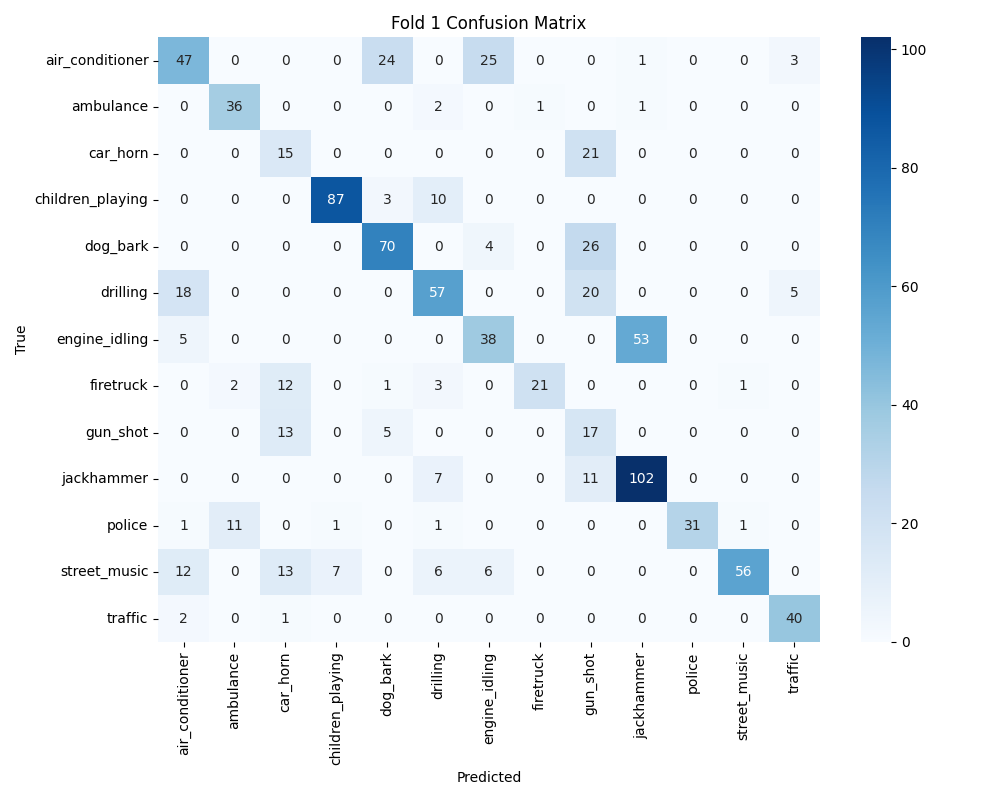
\includegraphics[width=\textwidth]{latex/assets/1-fold-1-epoch/confusion_matrix_simclr.png}
        \caption{SimCLR}
        \label{fig:cm_simclr}
    \end{subfigure}
    \hfill
    \begin{subfigure}[b]{0.24\textwidth}
        \centering
        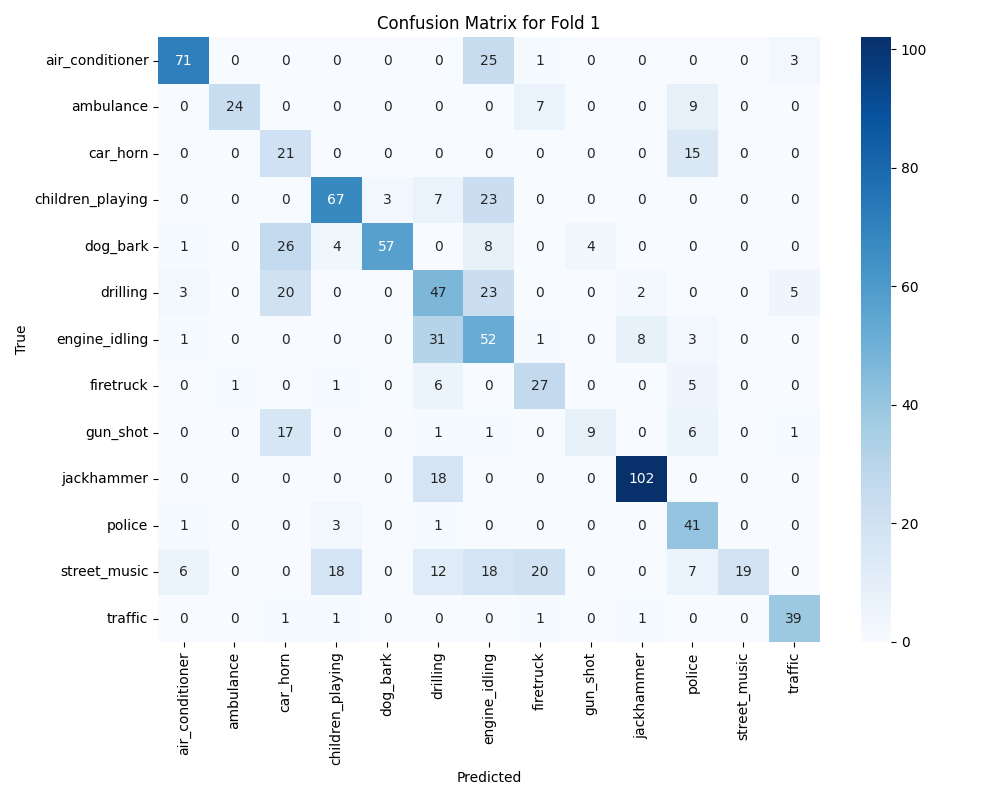
\includegraphics[width=\textwidth]{latex/assets/1-fold-1-epoch/confusion_matrix_mocov2.png}
        \caption{MoCo V2}
        \label{fig:cm_mocov2}
    \end{subfigure}
    \hfill
    \begin{subfigure}[b]{0.24\textwidth}
        \centering
        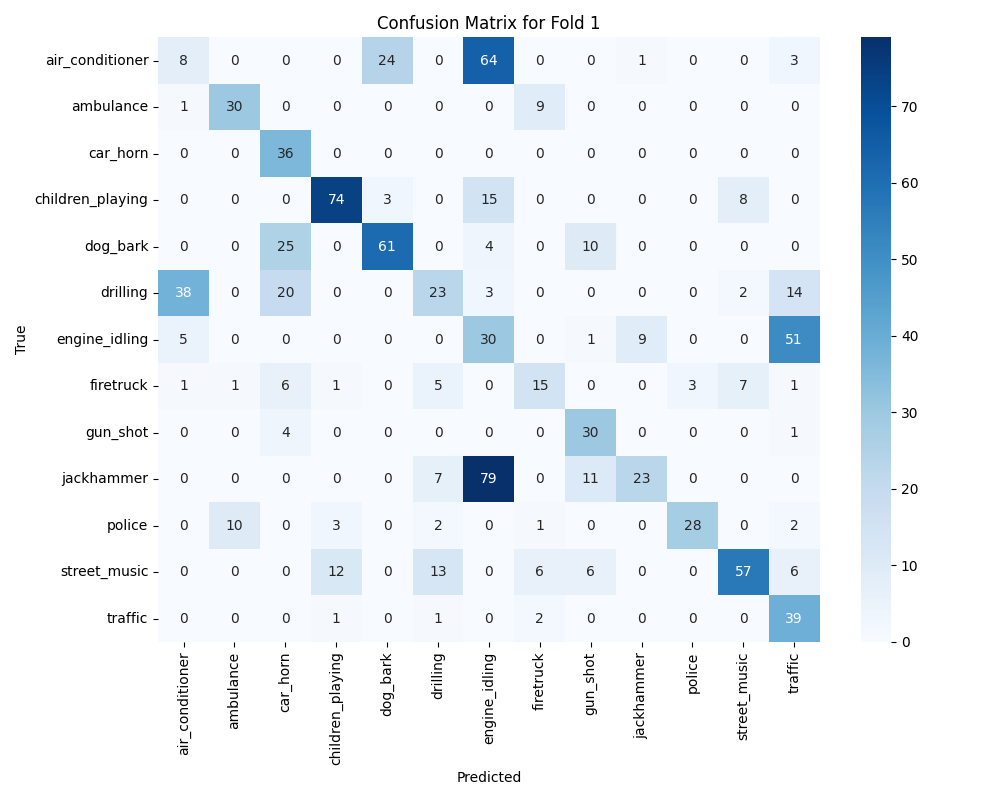
\includegraphics[width=\textwidth]{latex/assets/1-fold-1-epoch/confusion_matrix_moco.png}
        \caption{MoCo}
        \label{fig:cm_moco}
    \end{subfigure}
    \hfill
    \begin{subfigure}[b]{0.24\textwidth}
        \centering
        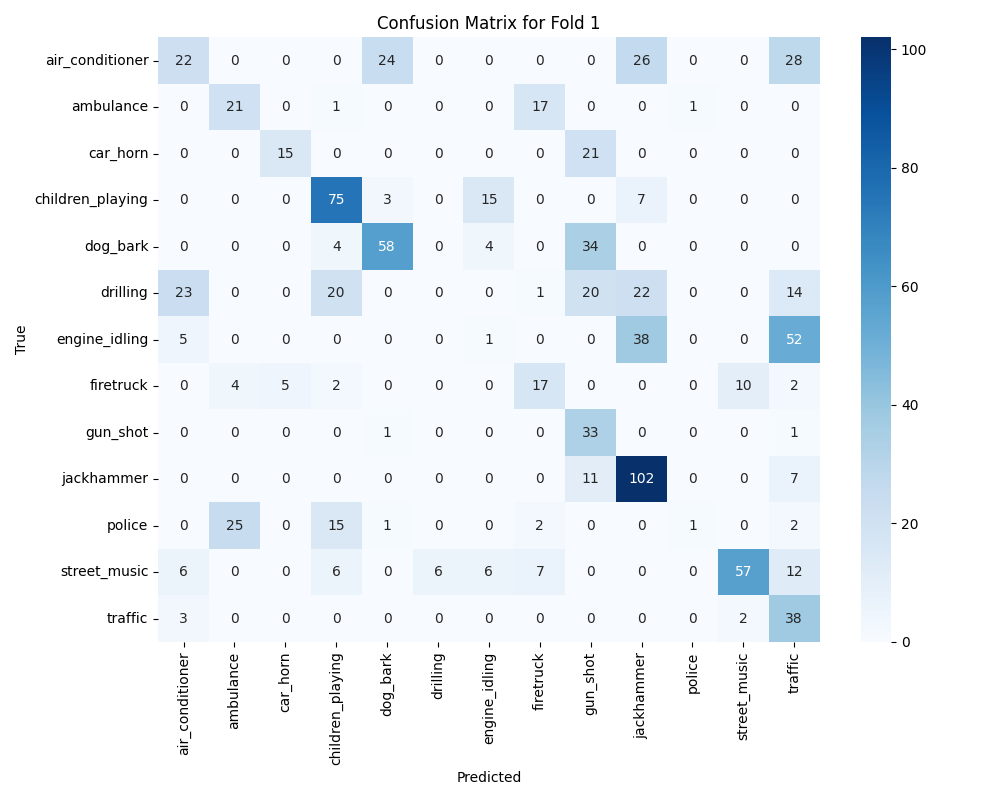
\includegraphics[width=\textwidth]{latex/assets/1-fold-1-epoch/confusion_matrix_byol.png}
        \caption{BYOL}
        \label{fig:cm_byol}
    \end{subfigure}
    
    \vspace{0.5cm}
    
    % Second row with 3 matrices (centered)
    \begin{subfigure}[b]{0.24\textwidth}
        \centering
        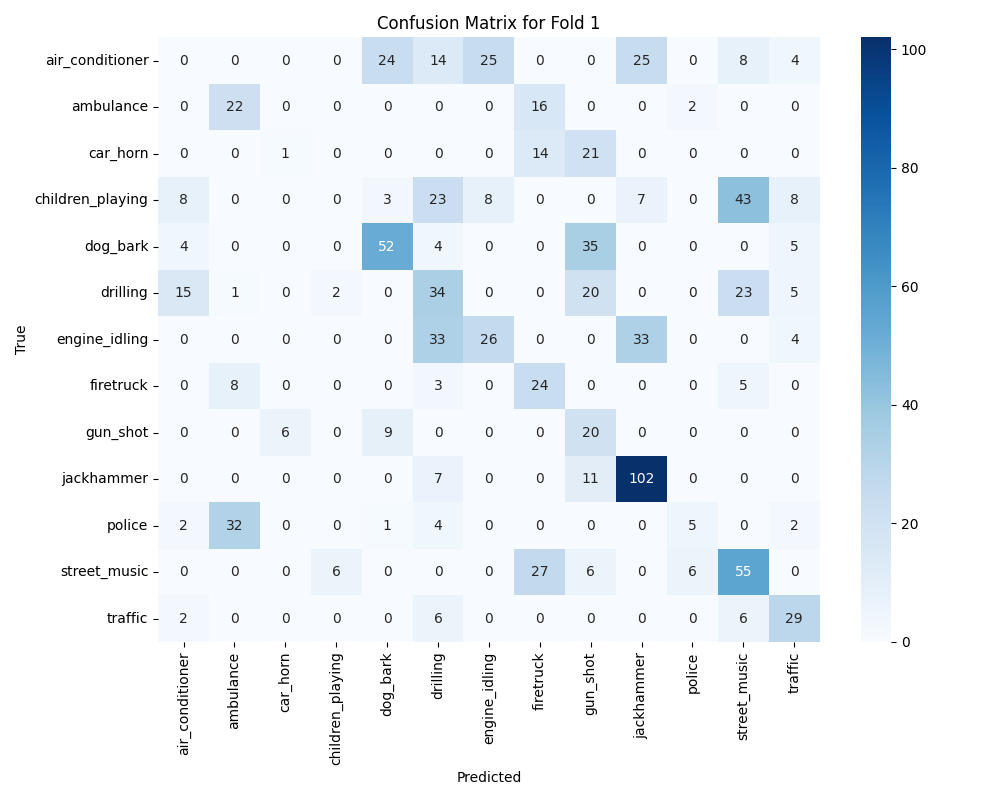
\includegraphics[width=\textwidth]{latex/assets/1-fold-1-epoch/confusion_matrix_swav.png}
        \caption{SwAV}
        \label{fig:cm_swav}
    \end{subfigure}
    \hfill
    \begin{subfigure}[b]{0.24\textwidth}
        \centering
        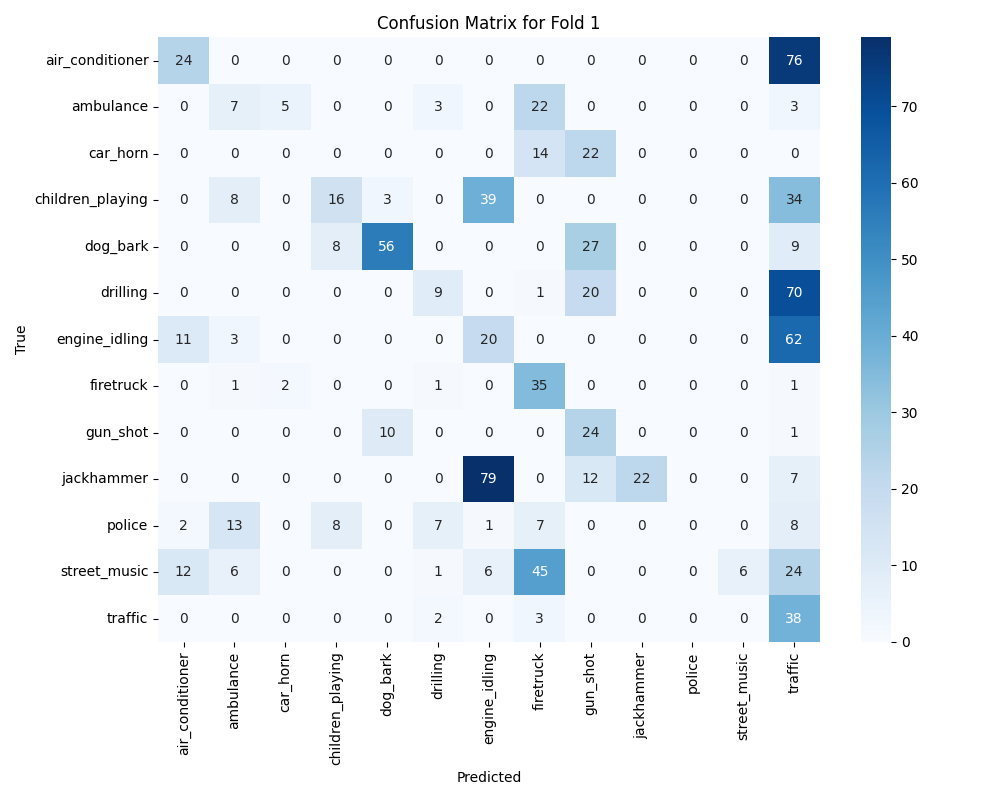
\includegraphics[width=\textwidth]{latex/assets/1-fold-1-epoch/confusion_matrix_dino.png}
        \caption{DINO}
        \label{fig:cm_dino}
    \end{subfigure}
    \hfill
    \begin{subfigure}[b]{0.24\textwidth}
        \centering
        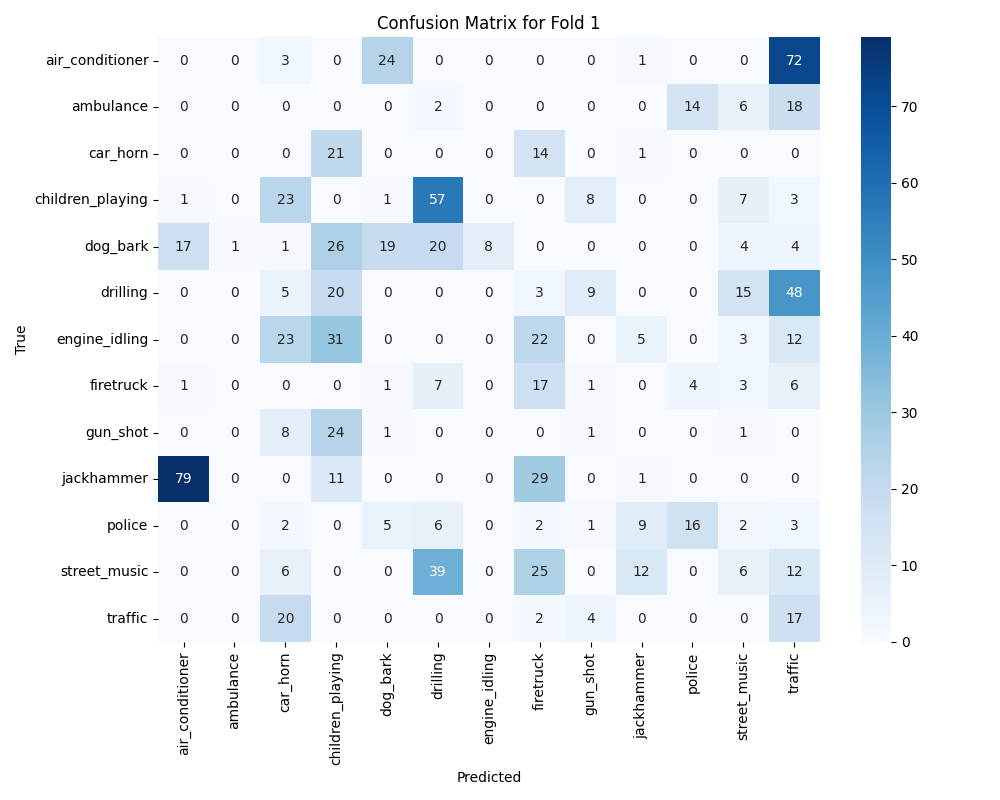
\includegraphics[width=\textwidth]{latex/assets/1-fold-1-epoch/confusion_matrix_barlow.png}
        \caption{Barlow Twins}
        \label{fig:cm_barlow}
    \end{subfigure}
    
    \caption{Confusion matrices for seven different SSL algorithms on the audio classification task.}
    \label{fig:all_confusion_matrices}
\end{figure*}
\subsubsection{SimCLR: Detailed Ablation}
\begin{table*}[ht]
    \centering
    \begin{tabular}{lcccccc}
    \toprule
    \textbf{Augmentation} & \textbf{Fold 1} & \textbf{Fold 2} & \textbf{Fold 3} & \textbf{Fold 4} & \textbf{Fold 5} & \textbf{Avg Acc(\%)} \\
    \midrule
    original & 21.34 & 16.17 & 11.29 & 16.33 & 8.27 & 14.77 \\
    noise\_5dB & 28.41 & 28.12 & 25.94 & 24.91 & 16.28 & 23.85 \\
    timestretch\_0.8 & 28.41 & 28.12 & 22.77 & 27.32 & 21.45 & 25.61 \\
    specaugment\_0 & 28.69 & 11.21 & 25.06 & 16.04 & 11.85 & 48.76 \\
    noise\_15dB & 27.91 & 22.92 & 25.94 & 24.19 & 16.28 & 23.85 \\
    patchaugment\_0 & 25.96 & 29.08 & 26.36 & 17.71 & -- & 24.06 \\
    specaugment\_1 & 29.71 & 15.61 & 19.86 & 25.62 & 14.77 & 20.42 \\
    pitchshift\_2 & 21.74 & 26.11 & 14.49 & 29.28 & 18.67 & 22.46 \\
    pitchshift\_-2 & 17.97 & 22.25 & 18.64 & 17.82 & -- & 19.67 \\
    specaugment\_2 & 23.06 & 15.87 & 22.60 & 27.19 & 10.75 & 19.89 \\
    timestretch\_1 & 23.61 & 20.58 & 21.05 & 25.06 & -- & 20.08 \\
    patchaugment\_1 & 25.90 & 26.77 & 21.12 & 22.40 & -- & 24.06 \\
    \bottomrule
    \end{tabular}
    \caption{Effect of Augmentations on Classification Accuracy: SimCLR}
\end{table*}
\begin{table*}[ht]
    \centering
    \begin{tabular}{ccc}
    \toprule
    \textbf{Project Output dim} & \textbf{Execution Time} & \textbf{Avg Accuracy} \\
    \midrule
    64 & 30 min & 81.02 \\
    128 & 31 min & 82.72 \\
    256 & 32 min & 80.68 \\
    \bottomrule
    \end{tabular}
    \caption{Effect of Projection Output Dimension on Performance: SimCLR}
\end{table*}

Some fold 5 data was cut off. We’ve marked these with “—” and calculated estimated mean accuracy only across available folds. This has the same evaluation procedure as MoCo , But the properties of either model's MoCo performance is far better since it maintains a dynamic memory bank for negative examples and SimClr needs larger batch size to generate sufficient negative examples. Other aspects also play key roles like with momentum encoder which gradually updates which makes is more stable , where we know the issue of small batches makes SimCLR collapse , with experiment we also observe that SimCLR takes significantly more gpu memory. These Significant reasons for our task in contrastive learning MOCO is far better. Keeping the eye on the above table Original data perform 14.77\% worst than augmented which shows that augmentation is have significant impact in representation learning , Time Stretch(0.8) perform better with 25.61 likely due to increasing temporal variability. Noise (5db) and Noise (15 db) are likely giving similar average accuracy. Due to limitation of time and resources we did not add any combination of augmentation unlike in Moco we added MixUp augmentation which also shows significant improvement.
The projection head in SimCLR maps high-dimensional representations to a lower-dimensional embedding space. This architectural component plays a crucial role in balancing information compression and expressiveness, which directly impacts downstream task performance.
Our investigation into different projection output dimensions (64, 128, and 256) was motivated by several theoretical considerations:
\begin{enumerate}
    \item Information compression: Smaller dimensions (64, 128) force the model to compress information into fewer dimensions, potentially leading to better generalization by capturing only the most essential features.
    \item Representation capacity: Larger dimensions (256, 512) can retain more information but risk overfitting, especially in low-data regimes like our audio classification task.
    \item Contrastive signal dilution: With higher dimensions, the contrastive signal might become diluted, potentially reducing discriminative power.
    \item Computational efficiency: Lower-dimensional projections require fewer computational resources during training and inference.
\end{enumerate}
Our experimental results align with these theoretical considerations. The performance improvement from 64 to 128 dimensions (81.02\% to 82.72\% accuracy) suggests that 64 dimensions were insufficient to encode the complex audio features needed for effective contrastive discrimination. However, the performance drop when increasing to 256 dimensions (80.68\% accuracy) indicates that larger projection spaces may be harder to optimize effectively with our limited computational resources and dataset size. This performance pattern suggests that 128 dimensions represents an optimal trade-off between expressiveness and generalization for our specific audio classification task. The smaller 64-dimensional space appears too restrictive, while the larger 256-dimensional space likely introduces optimization challenges and potential overfitting given our dataset constraints. These findings highlight the importance of carefully tuning the projection dimension in contrastive learning frameworks to balance information preservation with generalization capability.
\subsubsection{MoCo: Detailed Ablation}
\begin{table*}[ht]
    \centering
    \begin{tabular}{lcccccc}
    \toprule
    \textbf{Augmentation} & \textbf{Fold 1} & \textbf{Fold 2} & \textbf{Fold 3} & \textbf{Fold 4} & \textbf{Fold 5} & \textbf{Avg Acc(\%)} \\
    \midrule
    noise\_15dB & 67.58 & 64.11 & 66.67 & 63.00 & 57.79 & 63.15 \\
    noise\_5dB & 60.00 & 57.09 & 62.15 & 59.11 & 51.03 & 57.68 \\
    timestretch\_0.8 & 73.83 & 68.50 & 63.57 & 72.55 & 57.76 & 67.24 \\
    specaugment\_0 & 52.10 & 50.53 & 46.48 & 52.24 & 40.56 & 48.76 \\
    original & 64.72 & 64.66 & 56.56 & 59.01 & 49.85 & 58.96 \\
    patchaugment\_0 & 72.51 & 73.00 & 70.55 & 74.83 & 56.83 & 69.14 \\
    specaugment\_1 & 48.85 & 44.67 & 57.97 & 55.14 & 42.36 & 49.40 \\
    pitchshift\_2 & 71.08 & 66.89 & 67.71 & 74.00 & 62.18 & 68.37 \\
    pitchshift\_-2 & 72.50 & 69.43 & 70.44 & 71.58 & 57.91 & 68.37 \\
    specaugment\_2 & 55.51 & 47.23 & 51.07 & 51.82 & 41.22 & 49.77 \\
    timestretch\_1 & 68.98 & 71.83 & 65.63 & 72.04 & 61.54 & 68.04 \\
    patchaugment\_1 & 79.30 & 68.32 & 65.44 & 74.10 & 59.57 & 69.34 \\
    \bottomrule
    \end{tabular}
    \caption{Effect of Augmentations on Classification Accuracy: MoCo}
\end{table*}
\begin{table*}[ht]
    \centering
    \begin{tabular}{cccl}
    \toprule
    \textbf{Batch Size}& \textbf{Queue Length}& \textbf{Execution Time}&\textbf{Accuracy}\\
    \midrule
    8& 4096& 41 minutes&27\%\\
    16& 4096& 38 minutes&44\%\\
    32& 4096& 32 minutes&44\%\\
    32& 4096& 28 minutes&51\%\\
    \end{tabular}
    \caption{Batch Size and Queue Length Effect: MoCo}
\end{table*}

We  perform an evaluation study for each of the fold to check the effect of Augmentation Patchaugument\_1 consistently outperform other augmentations . Augmentations such as pitch shift and timestretch perform consistently better than specaugment and the original data. This is a typical observation as these augmentations help to add variability and help the model generalize better.
Patch Augmentation seems to have a particularly strong positive effect, potentially due to its ability to create robust variations of the data, which is critical for improving generalization across different folds.
We conduct an ablation study on the 5 fold to assess the effects of batch size and MoCo queue which took more than 5 hours , All the experiments are run on 2 Epochs only because limitation of time and computational resources available , increasing the batch size focus solely on the impact of architectural and training variations.
Increasing the batch size from 8 to 16 resulted in a dramatic gain in performance, suggesting that a larger batch size helps stabilize contrastive training. Interestingly, accuracy plateaued between batch sizes 16 and 32, indicating potential saturation of benefits with increased batch size alone.When increasing the MoCo queue size from 4096 to 8192 while keeping the batch size fixed at 32, we observed a notable performance gain of 7\%. This implies that a larger pool of negative samples shows the impact in representation learning, possibly by introducing greater semantic diversity and harder negatives during contrastive loss computation. While increasing the sequence length led to higher top-1 accuracy, a detailed inspection of the confusion matrix revealed that it caused more frequent misclassifications across classes. This indicates that although the model learned more global patterns from longer inputs, it may have overfit to certain dominant features or lost fine-grained distinctions between closely related classes.
The experiments highlight a subtle trade-off:
●	Longer sequence lengths boost raw accuracy, likely by capturing broader contextual information. However, they can also blur inter-class boundaries, leading to more misclassification — especially among acoustically similar classes.
●	Shorter sequences, while slightly lower in accuracy, may preserve discriminative temporal cues better, reducing confusion across categories.
We see the importance of balancing input granularity and contextual breadth in audio-based contrastive learning.
With the overall affiliation study results are strong and clearly show the value of certain augmentations and projections configuration. Our work lays the solid foundation but leaves behind significant areas for improvement to extend in future with deeper tuning, richer metric and alternative framework which are more advanced. Things that are not counted in this ablation study due to resource availability is Fixed projected head architecture, we only vary the projection head while keeping the MLP consistent , the architecture almost uses linear activations.


\end{document}
